
\documentclass[a4paper,12pt]{report}
\usepackage{a4wide}

%\documentclass[a5paper,10pt]{book}
%\usepackage[top=23mm, bottom=18mm, left=15mm, right=25mm]{geometry}
%\geometry{papersize={170mm,220mm}}


\usepackage[utf8x]{inputenc}
\usepackage[danish]{babel}

\usepackage{xr-hyper} %Externe hyper-ref
\usepackage[colorlinks=true, hyperindex=true, linkcolor=minmblaa, citecolor=minmblaa, urlcolor=minmblaa]{hyperref}
\hypersetup{colorlinks=true,filecolor=minmblaa,bookmarksnumbered=true} %Til hyperreferencer. Referencer med farver
\usepackage{needspace} % giver mulighed for at kræve at der skal være et antal tomme linier på siden før ellers indsættes et sideskift.
\usepackage{framed} %Bokse
\usepackage{wrapfig}

\usepackage{amsmath,amsfonts,amssymb,amsthm,mathtools} %Matematikpakker

\setlength{\parindent}{0mm} %Ingen Indhak i første linje i afsnit

\usepackage{color} %Farvepakke

\usepackage{array}
\usepackage{colortbl}
\usepackage{multirow} %Til at flette rækker i tabeller.

\usepackage{verbatim,mhchem}



	% DOWNLOAD FRA: http://sarovar.org/frs/?group_id=52&release_id=97
	% Læg i directory for hoved TEX fil
%\usepackage[draft]{pdfdraftcopy}
%\draftstring{Licens: Kasper Langt Mellemnavn Skårhøj}
%\draftfontsize{30}
	%\draftfontfamily{hlh}
	%\draftangle{45}
	%\definecolor{mycolor}{rgb}{.825,.855,1}
	%\draftcolor{mycolor}
	%\draftfontattrib



% = Sidehoved =
\usepackage{fancyhdr}
\pagestyle{fancy}
\renewcommand{\sectionmark}[1]{\markright{\protect\titlegraphic{dturoed}\textcolor{dtugraa}{\thesection~\MakeUppercase{#1}}}} % \thesection.\
\fancyhead{}
\fancyfoot{}
\fancyhead[R]{\titlefont\thepage}
\fancyhead[C]{}
\fancyhead[L]{\titlefont \small eNote \MakeUppercase{~\thechapter}~\hspace*{1ex}\rightmark}
\renewcommand\headrulewidth{0pt}
\fancypagestyle{plain}{\fancyfoot[C]{}}% {\titlefont\footnotesize\thepage}}
\setlength{\headheight}{15pt}


% = Længder
%\newlength{\envtblsep}\setlength{\envtblsep}{1\FrameSep}
\newlength{\obsl}\setlength{\obsl}{\textwidth-1.2cm-13.2pt}

% Includes:

% =     Fonts (select one)    =
\usepackage{mathpazo}\linespread{1.05} % Palatino needs more leading (space between lines)
\usepackage{bm} % bold math, must be loaded after the fontpackages

% % Til overskrifter
\DeclareTextFontCommand{\th}{\fontencoding{T1}\fontfamily{phv}\fontseries{b}\selectfont}
\newcommand\titlefont{\fontencoding{T1}\fontfamily{phv}\selectfont}


% =     PGF grafik      =
\usepackage{tikz}
\newcommand\titlegraphic[1]{%
\tikz[baseline] %
\draw[thick,color=#1]
(0pt  ,-0.25em) -- (0pt  ,0.85em)
(2.5pt,-0.25em) -- (2.5pt,0.85em)
(5pt  ,-0.25em) -- (5pt  ,0.85em)
(7.5pt,-0.25em) -- (7.5pt,0.85em);\hspace*{0.8ex} %
}

\newcommand\titlegraphicwide[1]{%
\tikz[baseline] %
\draw[line width=0.8mm,color=#1]
(0pt  ,-0.25em) -- (0pt  ,0.85em)
(4.5pt,-0.25em) -- (4.5pt,0.85em)
(9pt  ,-0.25em) -- (9pt  ,0.85em)
(13.5pt,-0.25em) -- (13.5pt,0.85em);\hspace*{0.8ex} %
}


% =      Title Layout      =
\usepackage{titlesec}
\makeatletter
\titleformat{\chapter}
	[display] % Shape
	{\titlefont\Huge\flushleft} % Title and label format
	{\titlefont\LARGE\bfseries \titlegraphicwide{dturoed}\textcolor{dtugraa}{\@chapapp~\thechapter}} % label
	{0.9em} % label/title separation
	{} % before code
	[] % after code
\makeatother
\titleformat{\section}
	[hang] % Shape
	{\titlefont\Large\flushleft} % Title and label format
	{\thesection} % label
	{0.9em} % label/title separation
	{} % before code
	[] % after code
\titleformat{\subsection}
	[hang] % Shape
	{\titlefont\large} % Title and label format
	{\thesubsection} % label
	{0.9em} % label/title separation
	{} % before code
	[] % after code
\titlespacing{\subsection}{0pt}{*6}{*1.5}
\titleformat{\subsubsection}
	[hang] % Shape
	{\titlefont} % Title and label format
	{\thesubsubsection} % label
	{0.9em} % label/title separation
	{} % before code
	[] % after code



% = Farver
\definecolor{dturoed}{rgb}{0.6, 0.0, 0.0}
\definecolor{dtugraa}{rgb}{0.5, 0.5, 0.5}	% Lidt mørkere. Korrekt = 0.4
\definecolor{mingroenstreg}{rgb}{0.4,0.8,0}	% Sekundærfarve 14 : 102/204/0	(Forårsgrøn) -> Eksempler
\definecolor{mingroen}{rgb}{0.32,0.64,0}		% Sekundærfarve 14, 80% mørkere (tekst)
\definecolor{minorangestreg}{rgb}{1,0.6,0}		% Sekundærfarve 1 : 255/153/0	(Orange) -> Opgaver
\definecolor{minorange}{rgb}{0.8,0.48,0}		% Sekundærfarve 1 , 80% mørkere (tekst)

\definecolor{minblaa}{rgb}{0.2,0.4,0.8}	% Sekundærfarve 13 , 51/102/204 	( Blå -> Definitioner etc)
\definecolor{minmblaa}{rgb}{0.16,0.32,0.64}	% Sekundærfarve 13 , 80% mørkere (tekst)
\definecolor{thmbackground}{rgb}{0.97,.97, 0.99}	% Farve 13 - lys baggrund

\definecolor{mingraastreg}{rgb}{.5,.5,.5}
\definecolor{hvadbackground}{rgb}{0.97,.97, 0.97}
\definecolor{sumgul}{rgb}{1,1,.8}

\definecolor{hjmopgfarve}{rgb}{.96,1,.96}


% = Counter
\newcounter{evncount}[chapter]
\setcounter{evncount}{0}
\renewcommand{\theevncount}{\thechapter.\arabic{evncount}}
\renewcommand{\theequation}{\thechapter-\arabic{equation}}


% = Eksempler = example =
\newenvironment{example}[1][]{
	\refstepcounter{evncount}
	\setlength{\obsl}{\textwidth-1.2cm-13.2pt-9pt} % fix width of the info envirnment%
	\def\FrameCommand{ 
		\textcolor{mingroenstreg}{\vrule width 4pt} 
		\hspace{5pt} 
	}%
	\MakeFramed{\advance\hsize-\width \FrameRestore}%
	\needspace{3\baselineskip}
	\titlegraphic{mingroen}
	\textcolor{mingroen}{
		\th{Eksempel \theevncount \hspace*{5mm} #1}
	} 
	\vspace*{3mm}%
	\begin{small}
	\par
}
{
	\end{small}
	\endMakeFramed
}


% = Opgaver = exercise =
\newenvironment{exercise}[1][]{
	\refstepcounter{evncount}
	\setlength{\obsl}{\textwidth-1.2cm-13.2pt-9pt}% fix width of the info envirnment%
	\def\FrameCommand{
		\textcolor{minorangestreg}{\vrule width 4pt}
		\hspace{5pt}
	}%
	\MakeFramed{\advance\hsize-\width \FrameRestore}%
	\needspace{3\baselineskip}
	\titlegraphic{minorange}
	\textcolor{minorange}{
		\th{Opgave \theevncount \hspace*{5mm} #1}
	} 
	\vspace*{3mm}%
	\begin{small}
	\par
}
{
	\end{small}
	\endMakeFramed
}


% = Bevis
\newenvironment{bevis}{
	\setlength{\obsl}{\textwidth-1.2cm-13.2pt-9pt} % fix width of the info envirnment%
	\def\FrameCommand{
		\textcolor{mingraastreg}{\vrule width 4pt} 
		\hspace{5pt}
	}%
	\MakeFramed{\advance\hsize-\width \FrameRestore}%
	\needspace{3\baselineskip}
	\titlegraphic{black}
	\textcolor{black}{
		\th{Bevis}
	}
	\vspace*{3mm}%
	\begin{small}
	\par
}
{
	\bevisslut 
	\end{small}
	\endMakeFramed
}


% = Definition =
\newenvironment{definition}[1][]{
	\vspace{4mm}
	\pagebreak[1]
	\setlength{\obsl}{\textwidth-1.2cm-2\FrameSep-13.2pt}%
	\def\FrameCommand{
		\fboxsep=\FrameSep\fcolorbox{minblaa}{thmbackground}
	}
	\begin{minipage}{\textwidth}
	\MakeFramed{\advance\hsize-\width\FrameRestore}
	\refstepcounter{evncount}
	\titlegraphic{minblaa}
	\textcolor{minmblaa}{
		\th{Definition \theevncount \hspace*{5mm} #1}
	}
	\vspace*{3mm}
	\par
}
{
	\endMakeFramed 
	\end{minipage}
	\vspace{4mm}
}


% = Theorem =
\newenvironment{theorem}[1][]{
	\vspace{4mm}
	\pagebreak[1]%
	\setlength{\obsl}{\textwidth-1.2cm-2\FrameSep-13.2pt}%
	\def\FrameCommand{
		\fboxsep=\FrameSep\fcolorbox{minblaa}{thmbackground}
	}%
	\begin{minipage}{\textwidth}
	\MakeFramed{\advance\hsize-\width\FrameRestore}%
	\refstepcounter{evncount}
	\titlegraphic{minblaa}
	\textcolor{minmblaa}{
		\th{Sætning \theevncount \hspace*{5mm} #1}
	}
	\vspace*{3mm}
	\par
}
{
	\endMakeFramed 
	\end{minipage}
	\vspace{4mm}
}


% = Lemma =
\newenvironment{lemma}[1][]{
	\vspace{4mm}
	\pagebreak[1]
	\setlength{\obsl}{\textwidth-1.2cm-2\FrameSep-13.2pt}%
	\def\FrameCommand{
		\fboxsep=\FrameSep \fcolorbox{minblaa}{thmbackground}
	}
	\begin{minipage}{\textwidth} 
	\MakeFramed{\advance\hsize-\width \FrameRestore}
	\refstepcounter{evncount}
	\titlegraphic{minblaa}
	\textcolor{minmblaa}{
		\th{Hjælpesætning \theevncount \hspace*{5mm} #1}
	}
	\vspace*{3mm}
	\par
}
{
	\endMakeFramed 
	\end{minipage}
	\vspace{4mm}
}


% = Corollary =
\newenvironment{corollary}[1][]{
	\vspace{4mm}
	\pagebreak[1]
	\setlength{\obsl}{\textwidth-1.2cm-2\FrameSep-13.2pt}%
	\def\FrameCommand{
		\fboxsep=\FrameSep \fcolorbox{minblaa}{thmbackground}
	}
	\begin{minipage}{\textwidth} 
	\MakeFramed{\advance\hsize-\width \FrameRestore}
	\refstepcounter{evncount}
	\titlegraphic{minblaa}
	\textcolor{minmblaa}{
		\th{Følgesætning \theevncount \hspace*{5mm} #1}
	}
	\vspace*{3mm}
	\par
}
{
	\endMakeFramed 
	\end{minipage}
	\vspace{4mm}
}


% = Metode = method
\newenvironment{method}[1][]{
	\vspace{4mm}
	\pagebreak[1]
	\setlength{\obsl}{\textwidth-1.2cm-2\FrameSep-13.2pt}%
	\def\FrameCommand{
		\fboxsep=\FrameSep \fcolorbox{black}{hvadbackground}
	}
	\begin{minipage}{\textwidth} 
	\MakeFramed{\advance\hsize-\width \FrameRestore}
	\refstepcounter{evncount}
	\titlegraphic{black}
	\textcolor{black}{
		\th{Metode \theevncount \hspace*{5mm} #1}
	}
	\vspace*{3mm}
	\par
}
{
	\endMakeFramed
	\end{minipage}
	\vspace{4mm}
}


% = Forklaring = explain =
\newenvironment{explain}[1][]{
	\vspace{4mm}
	\pagebreak[1]
	\setlength{\obsl}{\textwidth-1.2cm-2\FrameSep-13.2pt}%
	\def\FrameCommand{
		\fboxsep=\FrameSep \fcolorbox{black}{hvadbackground}
	}
	\MakeFramed{\advance\hsize-\width \FrameRestore}
	\refstepcounter{evncount}
	\titlegraphic{black}
	\textcolor{black}{
		\th{Forklaring \theevncount \hspace*{5mm} #1}
	}
	\vspace*{3mm}
	\par
}
{
	\endMakeFramed
	\vspace{4mm}
}


% = Bemærkning = remark =
\newenvironment{remark}[1][]{
	\vspace{4mm}
	\pagebreak[1]
	\setlength{\obsl}{\textwidth-1.2cm-2\FrameSep-13.2pt}%
	\def\FrameCommand{
		\fboxsep=\FrameSep \fcolorbox{black}{hvadbackground}
	}
	\begin{minipage}{\textwidth} 
	\MakeFramed{\advance\hsize-\width \FrameRestore}
	\refstepcounter{evncount}
	\titlegraphic{black}
	\textcolor{black}{
		\th{Bemærkning \theevncount \hspace*{5mm} #1}
	}
	\vspace*{3mm}
	\par
}
{
	\endMakeFramed 
	\end{minipage}
	\vspace{4mm}
}







% = OBS! = obs =
\newenvironment{obs}{\vspace{4mm}\par%
\begin{tabular}{m{1.2cm}<{\hspace*{2mm}}@{}|m{\obsl}@{}}\hspace*{-4pt}\raggedleft
\includegraphics[width=1.1cm]{../Strukturfiler/FIGS/Alert01} & \begin{minipage}{\obsl}}{\end{minipage}\\ \end{tabular}\vspace{4mm}\par}


% = INFO = info =
\newenvironment{info}{\vspace{4mm}\par%
\begin{tabular}{m{1.2cm}<{\hspace*{2mm}}@{}|m{\obsl}@{}}\hspace*{-4pt}\raggedleft
\includegraphics[width=1.1cm]{../Strukturfiler/FIGS/Info01} & \begin{minipage}{\obsl}}{\end{minipage}\\ \end{tabular}\vspace{4mm}\par}


% = THINK= think =
\newenvironment{think}{\vspace{4mm}\par%
\begin{tabular}{m{1.2cm}<{\hspace*{2mm}}@{}|m{\obsl}@{}}\hspace*{-4pt}\raggedleft
\includegraphics[width=0.7cm]{../Strukturfiler/FIGS/ChessPiece} & \begin{minipage}{\obsl}}{\end{minipage}\\ \end{tabular}\vspace{4mm}\par}


% = AHA= aha =
\newenvironment{aha}{\vspace{4mm}\par%
\begin{tabular}{m{1.2cm}<{\hspace*{2mm}}@{}|m{\obsl}@{}}\hspace*{-4pt}\raggedleft
\includegraphics[width=1.1cm]{../Strukturfiler/FIGS/Think} & \begin{minipage}{\obsl}}{\end{minipage}\\ \end{tabular}\vspace{4mm}\par}


% = BUILDUP= build =
\newenvironment{build}{\vspace{4mm}\par%
\begin{tabular}{m{1.2cm}<{\hspace*{2mm}}@{}|m{\obsl}@{}}\hspace*{-4pt}\raggedleft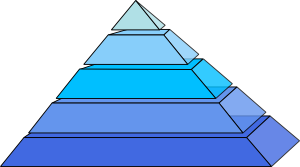
\includegraphics[width=1.1cm]{../Strukturfiler/FIGS/BluePyramid} & \begin{minipage}{\obsl}}{\end{minipage}\\ \end{tabular}\vspace{4mm}\newline}


% = Forudsætning = basis
\newenvironment{basis}{\begin{flushleft} \begin{itshape} }{\end{itshape} \end{flushleft}}


% = Opsummering =
\newenvironment{summary}{\clearpage\pagecolor{sumgul}\section{Opsummering}}{\newpage\pagecolor{white}}











% = Counter
\newcounter{opgavecount}[section]
\setcounter{opgavecount}{0}
\newcounter{spgcount}[opgavecount]
\setcounter{spgcount}{0}
\renewcommand{\thespgcount}{\alph{spgcount})}



% = EXERCISE = (DIVIDER)

\newcommand{\exercisebegin}[1][]{\bigskip\needspace{3\baselineskip}\refstepcounter{opgavecount}\titlegraphic{mingroen}\textcolor{mingroen}{\th{Opgave \theopgavecount \hspace*{1cm} #1}}\medskip\par}

% = QUIZEXERCISE = (DIVIDER)

\newcommand{\quizexercisebegin}[1][]{\bigskip\needspace{3\baselineskip}\refstepcounter{opgavecount}\titlegraphic{mingroen}\textcolor{mingroen}{\th{Quiz-Opgave \theopgavecount \hspace*{1cm} #1}}\medskip\par}

% = QUESTION =

\newenvironment{question}{\refstepcounter{spgcount}\begin{itemize}\item[\thespgcount]}{\end{itemize}\hspace*{\fill}}

% = VINK =

\newenvironment{vink}{\begin{tabular}{m{.9cm}<{\hspace*{2mm}}@{}|m{\obsl}@{}}\hspace*{-4pt}\raggedleft
\includegraphics[width=.9cm]{../Strukturfiler/FIGS/Think} & \begin{minipage}{\obsl}}{\end{minipage}\\ \end{tabular}\medskip\\}
	
% = FACIT =

\newenvironment{facit}{\begin{tabular}{m{.9cm}<{\hspace*{2mm}}@{}|m{\obsl}@{}}\hspace*{-4pt}\raggedleft
\includegraphics[width=.9cm]{../Strukturfiler/FIGS/Check} & \begin{minipage}{\obsl}}{\end{minipage}\\ \end{tabular}\medskip\\}








\newcommand{\afsnit}[1]{\bigskip\th{\titlegraphic{mingroen}\textcolor{mingroen}{#1}} \\ \rule[7pt]{.4\textwidth}{1pt} \vspace*{-2.5mm}\par}

% (DIVIDER):
\newcommand{\ugedagdatotitel}[4]{\pagebreak[4]\section{Semesteruge #1 -- #2 Dag \hspace*{1mm} (#3)} \vspace*{-4mm} \rule[5pt]{\textwidth}{1pt}\vspace*{-2.5mm} \begin{center}\large{\th{#4}}\end{center} \fancyhead[C]{\th{Semesteruge #1}}}

\newenvironment{skema}[1]{\definecolor{shadecolor}{rgb}{0.96,.98, 1.0} \setlength{\FrameSep}{6pt} \renewcommand{\FrameHeightAdjust}{10pt} \vspace*{-4pt}\begin{shaded} \begin{tabular}{#1}}{\end{tabular} \end{shaded} \vspace*{-7pt}}


% ========================

% MAKROER

%\newenvironment{matr}[1][]{\hspace*{-.8mm}\left[\hspace*{-1mm}\begin{array}{#1}}{\end{array}\hspace*{-1mm}\right]\hspace*{-.8mm}}
\newcommand{\bevisslut}{\begin{scriptsize} \begin{flushright} $ \blacksquare $ \end{flushright} \end{scriptsize}}

\newcommand{\tref}[2]{\hyperref[#1]{#2 \ref*{#1}}}
\newcommand{\thref}[2]{\hyperref[#1]{#2}}

\newcommand{\refA}[1]{\colorbox{yellow}{\ref{#1}}}
\newcommand{\hrefA}[2]{\colorbox{yellow}{\href{#1}{#2}}}
\newcommand{\trefA}[2]{\colorbox{yellow}{\hyperref[#1]{#2 \ref*{#1}}}}
\newcommand{\threfA}[2]{\colorbox{yellow}{\hyperref[#1]{#2}}}

\newenvironment{matr}[1]{\hspace*{-.8mm}\begin{bmatrix}\hspace*{-1mm}\begin{array}{#1}}{\end{array}\hspace*{-1mm}\end{bmatrix}\hspace*{-.8mm}}
\newcommand{\transp}{\hspace*{-.6mm}^{\top}}

\newcommand{\maengde}[2]{\left\lbrace \hspace*{-1mm} \begin{array}{c|c} #1 & #2 \end{array} \hspace*{-1mm} \right\rbrace}

\newenvironment{eqnalign}[1]{\setlength{\arraycolsep}{1.3pt}\begin{equation}\begin{array}{#1}}{\end{array}\end{equation}\par}
\newcommand{\eqnl}{\setlength{\arraycolsep}{1.3pt}}

\newcommand{\matind}[3]{{_\mathrm{#1}\mathbf{#2}_\mathrm{#3}}}
\newcommand{\vekind}[2]{{_\mathrm{#1}\mathbf{#2}}}
\newcommand{\jac}[2]{{\mathrm{Jacobi}_\mathbf{#1} (#2)}}
\newcommand{\diver}[2]{{\mathrm{div}\mathbf{#1} (#2)}}
\newcommand{\rot}[1]{{\mathbf{rot}\mathbf{(#1)}}}

\newcommand{\am}{\mathrm{am}}
\newcommand{\gm}{\mathrm{gm}}
\newcommand{\E}{\mathrm{E}}
\newcommand{\Span}{\mathrm{span}}
\newcommand{\mU}{\mathbf{U}}

\newcommand{\ms}{\medskip\\}
\newcommand{\bs}{\bigskip\\}

\newcommand{\mA}{\mathbf{A}}
\newcommand{\mB}{\mathbf{B}}
\newcommand{\mC}{\mathbf{C}}
\newcommand{\mD}{\mathbf{D}}
\newcommand{\mE}{\mathbf{E}}
\newcommand{\mF}{\mathbf{F}}
\newcommand{\mK}{\mathbf{K}}
\newcommand{\mI}{\mathbf{I}}
\newcommand{\mM}{\mathbf{M}}
\newcommand{\mN}{\mathbf{N}}
\newcommand{\mQ}{\mathbf{Q}}
\newcommand{\mT}{\mathbf{T}}
\newcommand{\mV}{\mathbf{V}}
\newcommand{\mW}{\mathbf{W}}
\newcommand{\mX}{\mathbf{X}}
\newcommand{\ma}{\mathbf{a}}
\newcommand{\mb}{\mathbf{b}}
\newcommand{\mc}{\mathbf{c}}
\newcommand{\md}{\mathbf{d}}
\newcommand{\me}{\mathbf{e}}
\newcommand{\mn}{\mathbf{n}}
\newcommand{\mr}{\mathbf{r}}
\newcommand{\mv}{\mathbf{v}}
\newcommand{\mw}{\mathbf{w}}
\newcommand{\mx}{\mathbf{x}}
\newcommand{\mxb}{\mathbf{x_{bet}}}
\newcommand{\my}{\mathbf{y}}
\newcommand{\mz}{\mathbf{z}}
\newcommand{\reel}{\mathbb{R}}
\newcommand{\mL}{\bm{\Lambda}} %Lambda-matrix
\newcommand{\mnul}{\bm{0}}
\newcommand{\trap}[1]{\mathrm{trap}(#1)}
\newcommand{\Det}{\operatorname{Det}}
\newcommand{\adj}{\operatorname{adj}}
\newcommand{\Ar}{\operatorname{Areal}}
\newcommand{\Vol}{\operatorname{Vol}}
\newcommand{\Rum}{\operatorname{Rum}}
\newcommand{\diag}{\operatorname{\bf{diag}}}
\newcommand{\bidiag}{\operatorname{\bf{bidiag}}}
\newcommand{\spanVec}[1]{\mathrm{span}\{#1\}}
\newcommand{\Div}{\operatorname{Div}}
\newcommand{\Rot}{\operatorname{\mathbf{Rot}}}

\newcommand{\Jac}{\operatorname{Jacobi}}
\newcommand{\Tan}{\operatorname{Tan}}
\newcommand{\Ort}{\operatorname{Ort}}
\newcommand{\Flux}{\operatorname{Flux}}
\newcommand{\Cmass}{\operatorname{Cm}}
\newcommand{\Imom}{\operatorname{Im}}
\newcommand{\Pmom}{\operatorname{Pm}}
\newcommand{\IS}{\operatorname{I}}
\newcommand{\IIS}{\operatorname{II}}
\newcommand{\IIIS}{\operatorname{III}}
\newcommand{\Le}{\operatorname{L}}
\newcommand{\app}{\operatorname{app}}
\newcommand{\M}{\operatorname{M}}
\newcommand{\re}{\mathrm{Re}}
\newcommand{\im}{\mathrm{Im}}

\newcommand{\compl}{\mathbb{C}} %de komplekse tal
\newcommand{\e}{\mathrm{e}} %eksponentialfunktionen. lodret 'e', og altså ikke kursiv ligesom andre bogstaver.





% Medialink: SCREEN: (QRcode) + thumbnail image + link på kodenummer (til qr.dtu.dk)
\newcommand{\onlinemedia}[3]{
	\begin{wrapfigure}{r}{3.2cm} 
		\vspace{-30pt} 
		\vspace{#1pt} 
		\begin{flushright} 
			\includegraphics[width=3cm]{qr/#2.png} 
			\tiny 
			\href{http://qr.dtu.dk/#2}{#2: #3}
			\normalsize  
		\end{flushright} 
		\vspace{-10pt} 
	\end{wrapfigure}
}
\newcommand{\onlinemediathumb}[3]{
	\begin{wrapfigure}{r}{3.2cm} 
		\vspace{-30pt} 
		\vspace{#1pt} 
		\begin{flushright} 
			\includegraphics[width=3cm]{qr/#2.png} 
			\includegraphics[width=3cm]{qr/#2_thumb.png} 
			\tiny 
			\href{http://qr.dtu.dk/#2}{#2: #3}
			\normalsize  
		\end{flushright} 
		\vspace{-10pt} 
	\end{wrapfigure}
}



% Index:
\usepackage{makeidx}
\makeindex
\newcommand\ind[2]{\index{#1}\textbf{\textit{\textcolor{black}{#2}}}}

% ###SERVER_EXCLUDE_BEGIN###
\externaldocument[NUID17-]{../../enoten/TN01-Talrum/Talrum}
\externaldocument[NUID1-]{../../enoten/TN02-Ligningssystemer/TNdriver}
\externaldocument[NUID2-]{../../enoten/TN03-Matricer_og_Matrixalgebra/Matricer_og_matrixalgebra}
\externaldocument[NUID3-]{../../enoten/TN04-Kvadratiske_matricer/TNdriver}
\externaldocument[NUID11-]{../../enoten/TN05-Determinanter/Determinanter}
\externaldocument[NUID12-]{../../enoten/TN06-GeometriskeVektorer/GeometriskeVektorer}
\externaldocument[NUID18-]{../../enoten/TN07-Vektorrum/VektorRum}
\externaldocument[NUID21-]{../../enoten/TN08-LinAfbildninger/LinAfbildninger}
\externaldocument[NUID23-]{../../enoten/TN09-Egenvaerdier_og_egenvektorer/TNdriver}
\externaldocument[NUID24-]{../../enoten/TN10-Diagonalisering_med_egenvektorer/TNdriver}
\externaldocument[NUID10-]{../../enoten/TN11-1.ordens_differentialligninger/TNdriver}
\externaldocument[NUID13-]{../../enoten/TN12-1.ordens_differentialligningssystemer/TNdriver}
\externaldocument[NUID14-]{../../enoten/TN13-2.ordens_differentialligninger/TNdriver}
\externaldocument[NUID27-]{../../enoten/TN14-Elemenataere_funktioner/Elementaere_Funktioner}
\externaldocument[NUID28-]{../../enoten/TN15-Funktioner2Variable/Funktioner_To_Variable}
\externaldocument[NUID29-]{../../enoten/TN16-Gradienter_og_Tangentplaner/Gradienter_og_Tangentplaner}
\externaldocument[NUID32-]{../../enoten/TN17-Taylor_formler/Taylor_Formler}
\externaldocument[NUID33-]{../../enoten/TN18-Taylor_2Var/Taylor_2Var}
\externaldocument[NUID34-]{../../enoten/TN19-SymMat/SymmetriskeMatricer}
\externaldocument[NUID35-]{../../enoten/TN20-KegleSnit/Keglesnit}
\externaldocument[NUID36-]{../../enoten/TN21-Riemann_Integral/Riemann_01}
\externaldocument[NUID37-]{../../enoten/TN22-Plan_Int/Plan_Int_01}
\externaldocument[NUID39-]{../../enoten/TN23-Flade_Int/Flade_Rum_Int_01}
\externaldocument[NUID40-]{../../enoten/TN24-Vektorfelter/Vektorfelter_01}
\externaldocument[NUID41-]{../../enoten/TN25-Flux/Flux_02}
\externaldocument[NUID42-]{../../enoten/TN26-Gauss/Gauss_01}
\externaldocument[NUID128-]{../../enoten/TN27-Stokes/Stokes_01}
\externaldocument[NUID43-]{../../enoten/TN29-KomplekseTal/KomplekseTal}

\externaldocument[NUID6-]{../../E-math-opgaver/Opgaver/opgU123}
\externaldocument[NUID19-]{../../E-math-opgaver/Opgaver/opgU45}
\externaldocument[NUID20-]{../../E-math-opgaver/Opgaver/opgU678}
\externaldocument[NUID25-]{../../E-math-opgaver/Opgaver/opgU910SD}
\externaldocument[NUID31-]{../../E-math-opgaver/OpgaverF11-U123/opgF123}
% \externaldocument[NUID9-]{../../E-math-opgaver/Opgaver/Dagsordner E10}
% ###SERVER_EXCLUDE_END###


% Begin document and set alternative chapter title:
\begin{document}
\renewcommand{\chaptername}{eNote}

\setcounter{chapter}{24} %SÆT DETTE TAL TIL 1 MINDRE END DET AKTUELLE TRANSFERNOTE-NUMMER!!

%%%%%%%%%%%%%%%%%%%%%%%%55%%%%%%%%%%%%%%%%%%%%%
%%%%%%%%%%%%%%%%%%%%%%%%%%%%%%%%%%%%%%%%%%%%%
%%% HERFRA SKAL DU SKRIVE ELLER INDSÆTTE %%%%
%%% DEN FIL DU ØNSKER %%%%%%%%%%%%%%%%%%%%%%%
%%%%%%%%%%%%%%%%%%%%%%%%%%%%%%%%%%%%%%%%%%%%%
%%%%%%%%%%%%%%%%%%%%%%%%%%%%%%%%%%%%%%%%%%%%%

% REF: TransferNote \ref{TN4-tn4} \nameref{TN4-tn4}
%
% \tref{NUID14-thm.koma}{sætning} \tref{NUID28-tn15}{eNote}
%
%\tref{NUID34-tn19}{eNote} Symmetriske matricer
%\tref{NUID33-tn18}{eNote} Taylor i 2 variable
%
% 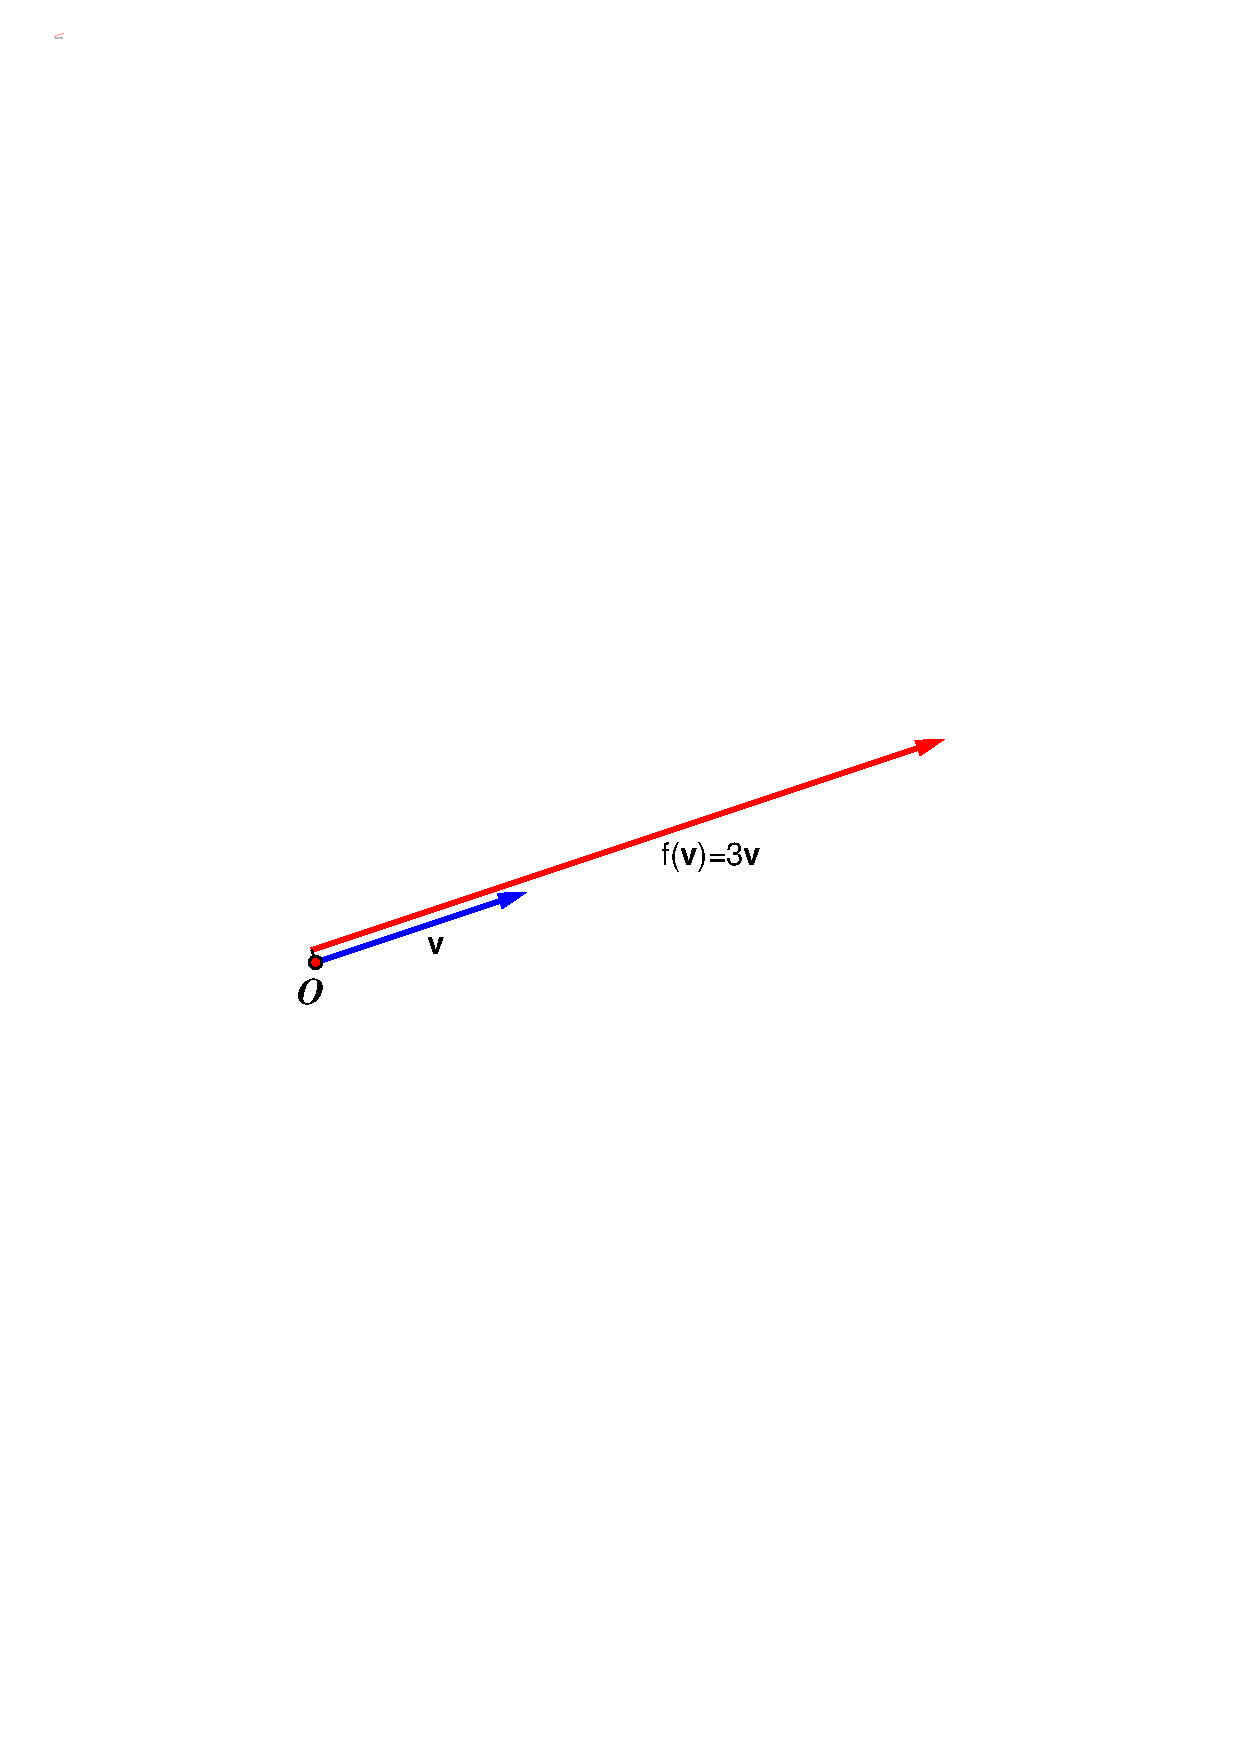
\includegraphics[trim=5cm 12cm 5cm 12cm,width=0.40\textwidth,clip]{skalering.pdf}
%
%\begin{equation}
%\matind vMa \cdot \matind aFa \cdot \matind aMv = \matind vFv \, ,
%\end{equation}
%hvor
%\begin{equation}
%\matind aMv = \begin{matr}{cccc} \vekind av_1 & \vekind av_2 & \cdots & \vekind av_n \end{matr} \quad \mathrm{og} \quad %\matind vFv = \diag(\lambda_1, \lambda_2, \ldots, \lambda_n) \, .
%\end{equation}
%
%$\vekind{e}{F}$
%$\matind{e}{F}{w}$
%
%\href{http://www-groups.dcs.st-and.ac.uk/~history/}{http://www-groups.dcs.st-and.ac.uk/~history/}

%%%%%%%%%%%%%%%%%%%%%%%%%%%%%%%%%%%%%%%%%%%%%%%%%%%
%%%%%%%%%%%%%%%%%%%%%%%%%%%%%%%%%%%%%%%%%%%%%%%%%%%
%%%%%%%%%%%%%%%%%%%%%%%%%%%%%%%%%%%%%%%%%%%%%%%%%%%
%%%%%%%%%%%%%%%%%%%%%%%%%%%%%%%%%%%%%%%%%%%%%%%%%%%

\chapter{Vektorfelter langs kurver} \label{tn25}


\begin{basis}
I \tref{NUID40-tn24}{eNote} dyrkes de indledende overvejelser om vektorfelter. I denne eNote vil vi se på vektorfelternes værdier langs kurver og benytte metoder fra  \tref{NUID37-tn22}{eNote} om kurveintegration til at opstille de såkaldte tangentielle kurveintegraler og bruge dem til at undersøge om et givet vektorfelt er et gradientvektorfelt eller ej. Hvis et vektorfelt er et gradientvektorfelt for en funktion $f(x,y,z)$ så kan vi konstruere alle sådanne stamfunktioner ved hjælp af tangentiel kurveintegration af vektorfeltet. Og som vi skal se, gælder det også omvendt, at hvis det tangentielle kurveintegral af et givet vektorfeltet over enhver lukket kurve er $0$, så er vektorfeltet et gradientvektorfelt. Det tangentielle kurveintegral af et vektorfelt over en lukket kurve kaldes cirkulationen af vektorfeltet over kurven. Alene ud fra navnet er det ikke overraskende, at en sådan generel cirkulation $0$ er ækvivalent med, at vektorfeltet selv har rotationsvektorfeltet $\mathbf{0}$.
\end{basis}




%%%%%%%%%%%%%%%%%%%%%%%%%%%%%%%%%%%%%%%%%%%%%%%%%%%
%%%%%%%%%%%%%%%%%%%%%%%%%%%%%%%%%%%%%%%%%%%%%%%%%%%
%%%%%%%%%%%%%%%%%%%%%%%%%%%%%%%%%%%%%%%%%%%%%%%%%%%
%%%%%%%%%%%%%%%%%%%%%%%%%%%%%%%%%%%%%%%%%%%%%%%%%%%
%%%%%%%%%%%%%%%%%%%%%%%%%%%%%%%%%%%%%%%%%%%%%%%%%%%%%%%%%%%%%%%%%%%%%%%%%%%%%%%%%%%%%
%%%%%%%%%%%%%%%%%%%%%%%%%%%%%%%%%%%%%%%%%%%%%%%%%%%%%%%%%%%%%%%%%%%%%%%%%%%%%%%%%%%%%

\section{Det tangentielle kurveintegral} \label{secTangKurveInt}
Lad ${\bf V}(x,y,z)$ være et glat vektorfelt i rummet, se \tref{NUID40-tn24}{eNote} og lad
$K_{\bf r}$ betegne en glat parametriseret kurve:
\begin{equation}
K_{\bf r} \quad : \quad \mathbf{r}(u) = (x(u), y(u), z(u)) \quad , \quad u \in [a, b] \quad.
\end{equation}
Langs med kurven $K_{\bf r}$ har vi så -- i ethvert punkt $\mathbf{r}(u)$ på kurven --  \emph{to} vektorer, dels vektorfeltets værdi i
punktet, ${\bf V}(\mathbf{r}(u))$, og dels tangentvektoren $\mathbf{r}'(u)$ til kurven i punktet. Ved hjælp af disse to vektorer kan vi konstruere en glat funktion på kurven, som derefter kan integreres over kurven: \\


Det {\em tangentielle kurveintegral} af ${\bf
V}(x,y,z)$ langs en given parametriseret kurve $K_{\bf r}$ er
kurve\-in\-te\-gralet af længden af \emph{projektionen} (med fortegn) af ${\bf V}({\bf
r}(u))$ på kurvens tangent der er repræsenteret ved ${\bf r}'(u)$. \\

Det ønskede integral er altså defineret således:

\begin{definition}
Det tangentielle kurveintegral af ${\bf
V}(x,y,z)$ langs $K_{\bf r}$ er defineret ved:
\begin{equation}
\Tan({\bf V}, K_{\bf r})\, = \, \int_{K_{\bf r}}{\bf V} \bm{\cdot} {\bf e}\,\,d\mu \quad .
\end{equation}
\end{definition}

Integranden er altså i dette tilfælde givet
ved skalarproduktet:
\begin{equation}
f({\bf r}(u)) \, = \, {\bf V}({\bf r}(u))\cdot {\bf e}(u) \quad ,
\end{equation}
hvor ${\bf e}(u)$ er defineret ved
\begin{equation}
{\bf e}(u)\, = \,
\begin{cases}
&{\bf r}'(u)/ \Vert {\bf r}'(u) \Vert  \quad \text{hvis}\quad {\bf r}'(u)\,
\neq \,
{\bf 0} \\
&{\bf 0} \quad \text{hvis} \quad {\bf r}'(u)\, = \, {\bf 0} \quad
.
\end{cases}
\end{equation}
Bemærk, at så har vi for alle $u$:
\begin{equation}
{\bf e}(u)\,\Vert {\bf r}'(u) \Vert \, = \, {\bf r}'(u) \quad .
\end{equation}


Det {tangentielle kurveintegral} $\Tan({\bf V}, K_{\bf r})$ af ${\bf
V}$ langs $K_{\bf r}$ er derfor relativt simpelt at \emph{udregne} - vi
behøver faktisk ikke først at finde Jacobi-funktionen $\,\Jac_{\mathbf{r}}(u)\,$, altså
\emph{længden} af ${\bf r}'(u)$ :
\begin{equation} \label{eqTan}
\begin{aligned}
\Tan({\bf V}, K_{\bf r})\, &= \, \int_{K_{\bf r}}{\bf V}\bm{\cdot} {\bf e}\,\,d\mu \,\\
 &= \, \int_{a}^{b}\left({\bf
V}({\bf r}(u))\bm{\cdot} {\bf e}(u)\right) \, \Jac_{\mathbf{r}}(u) \,du \,\\
&= \, \int_{a}^{b}{\bf
V}({\bf r}(u))\bm{\cdot} \left({\bf e}(u)\,\Vert {\bf r}'(u) \Vert \right) \,du \,\\
 &=
\, \int_{a}^{b}{\bf V}({\bf r}(u))\bm{\cdot} {\bf r}'(u)\,\,du \quad .
\end{aligned}
\end{equation}

Vi har altså følgende simple udtryk for tangentielle kurveintegraler:

\begin{theorem}
Det tangentielle kurveintegral af ${\bf
V}(x,y,z)$ langs $K_{\bf r}$ kan \emph{beregnes} således:
\begin{equation}
\Tan({\bf V}, K_{\bf r})\, = \,  \int_{K_{\bf r}}{\bf V} \bm{\cdot} {\bf e}\,\,d\mu   \, = \, \int_{a}^{b}{\bf V}({\bf r}(u))\bm{\cdot} {\bf r}'(u)\,\,du \quad .
\end{equation}
\end{theorem}



\begin{aha}
Læg mærke til, at den sidste integrand i (\ref{eqTan}) er kontinuert når
${\bf V}(x,y,z)$ og ${\bf r}'(u)$ er kontinuerte selv om det ikke
umiddelbart fremgår af definitionen (vektorfeltet ${\bf e}(u)$ er jo
ikke nødvendigvis kontinuert - medmindre ${\bf r}(u)$ er en re\-gu\-lær
parameterfremstilling).
\end{aha}





\begin{think}
Hvis kurven gennemløbes baglæns, så skifter $\Tan({\bf V}, K_{\bf r})$ fortegn. \\

 Lad nemlig
\begin{equation}
\overline{K}_{\overline{\bf r}} \quad : \quad \overline{\bf r}(u) = \mathbf{r}(b+a-u) \quad , \quad u \in [a, b] \quad .
\end{equation}
Så er $\overline{{\bf r}}'(u) = - {\bf r}'(u)$ og $\overline{{\bf e}}(u) = - {\bf e}(u)$ sådan at
\begin{equation}
\Tan({\bf V}, \overline{K}_{\overline{\bf r}}) = -\Tan({\bf V}, K_{\bf r}) \quad .
\end{equation}
\end{think}

\begin{definition}
I analogi med det tangentielle kurveintegral definerer vi det {\em ortogonale} kurveintegral
$\Ort({\bf V}, K_{\bf r})$ af ${\bf V}$ langs $K_{\bf r}$ ved at
projicere ${\bf V}({\bf r}(u))$ vinkelret ind på den plan i rummet, som selv står
vinkelret på ${\bf r}'(u)$ og dernæst finde kurveintegralet af
længden af den projektion (som funktion af $u$).
\end{definition}




\begin{example}
Lad $\, {\bf V}(x,y,z)\, = \, (0, z, y) \,$. Vi ønsker at bestemme
det tangentielle kurveintegral af ${\bf V}$ langs følgende
parametriserede stykke af en skruelinje
\begin{equation}K_{\bf r}: \,\, {\bf
r}(u) \, = \, \left(\cos(u), \,\sin(u),\, u\right), \, \, \, u \in
\left[0, \frac{\pi}{2}\right]\quad .
\end{equation}
Ved at indsætte i (\ref{eqTan}) fås
\begin{equation}
\begin{aligned}
\Tan({\bf V}, K_{\bf r})\, &= \,\int_{0}^{\pi/2}{\bf V}({\bf
r}(u))\cdot {\bf r}'(u)\,du \, \\ &= \, \int_{0}^{\pi/2}(0, u,
\sin(u))\cdot (-\sin(u), \cos(u), 1)\,du \, \\ &= \,
\int_{0}^{\pi/2}(u\cos(u) + \sin(u))\,du \, \\ &= \,
[u\sin(u)]_{0}^{\pi/2} \, = \, \frac{\pi}{2}\quad .
\end{aligned}
\end{equation}
\end{example}

\begin{exercise}
Lad $\, {\bf V}(x,y,z)\, = \, (0, x, z) \,$. Bestem både det
tangentielle og det ortogonale kurveintegral af ${\bf V}$ langs
følgende parametriserede stykke af en cirkel
\begin{equation}
K_{\bf r}: \,\, {\bf
r}(u) \, = \, \left(\cos(u), \,\sin(u),\, 0\right), \, \, \, u \in
\left[ 0, \frac{\pi}{2}\right]\quad .
\end{equation}
\end{exercise}


\begin{figure}[t]
\centerline{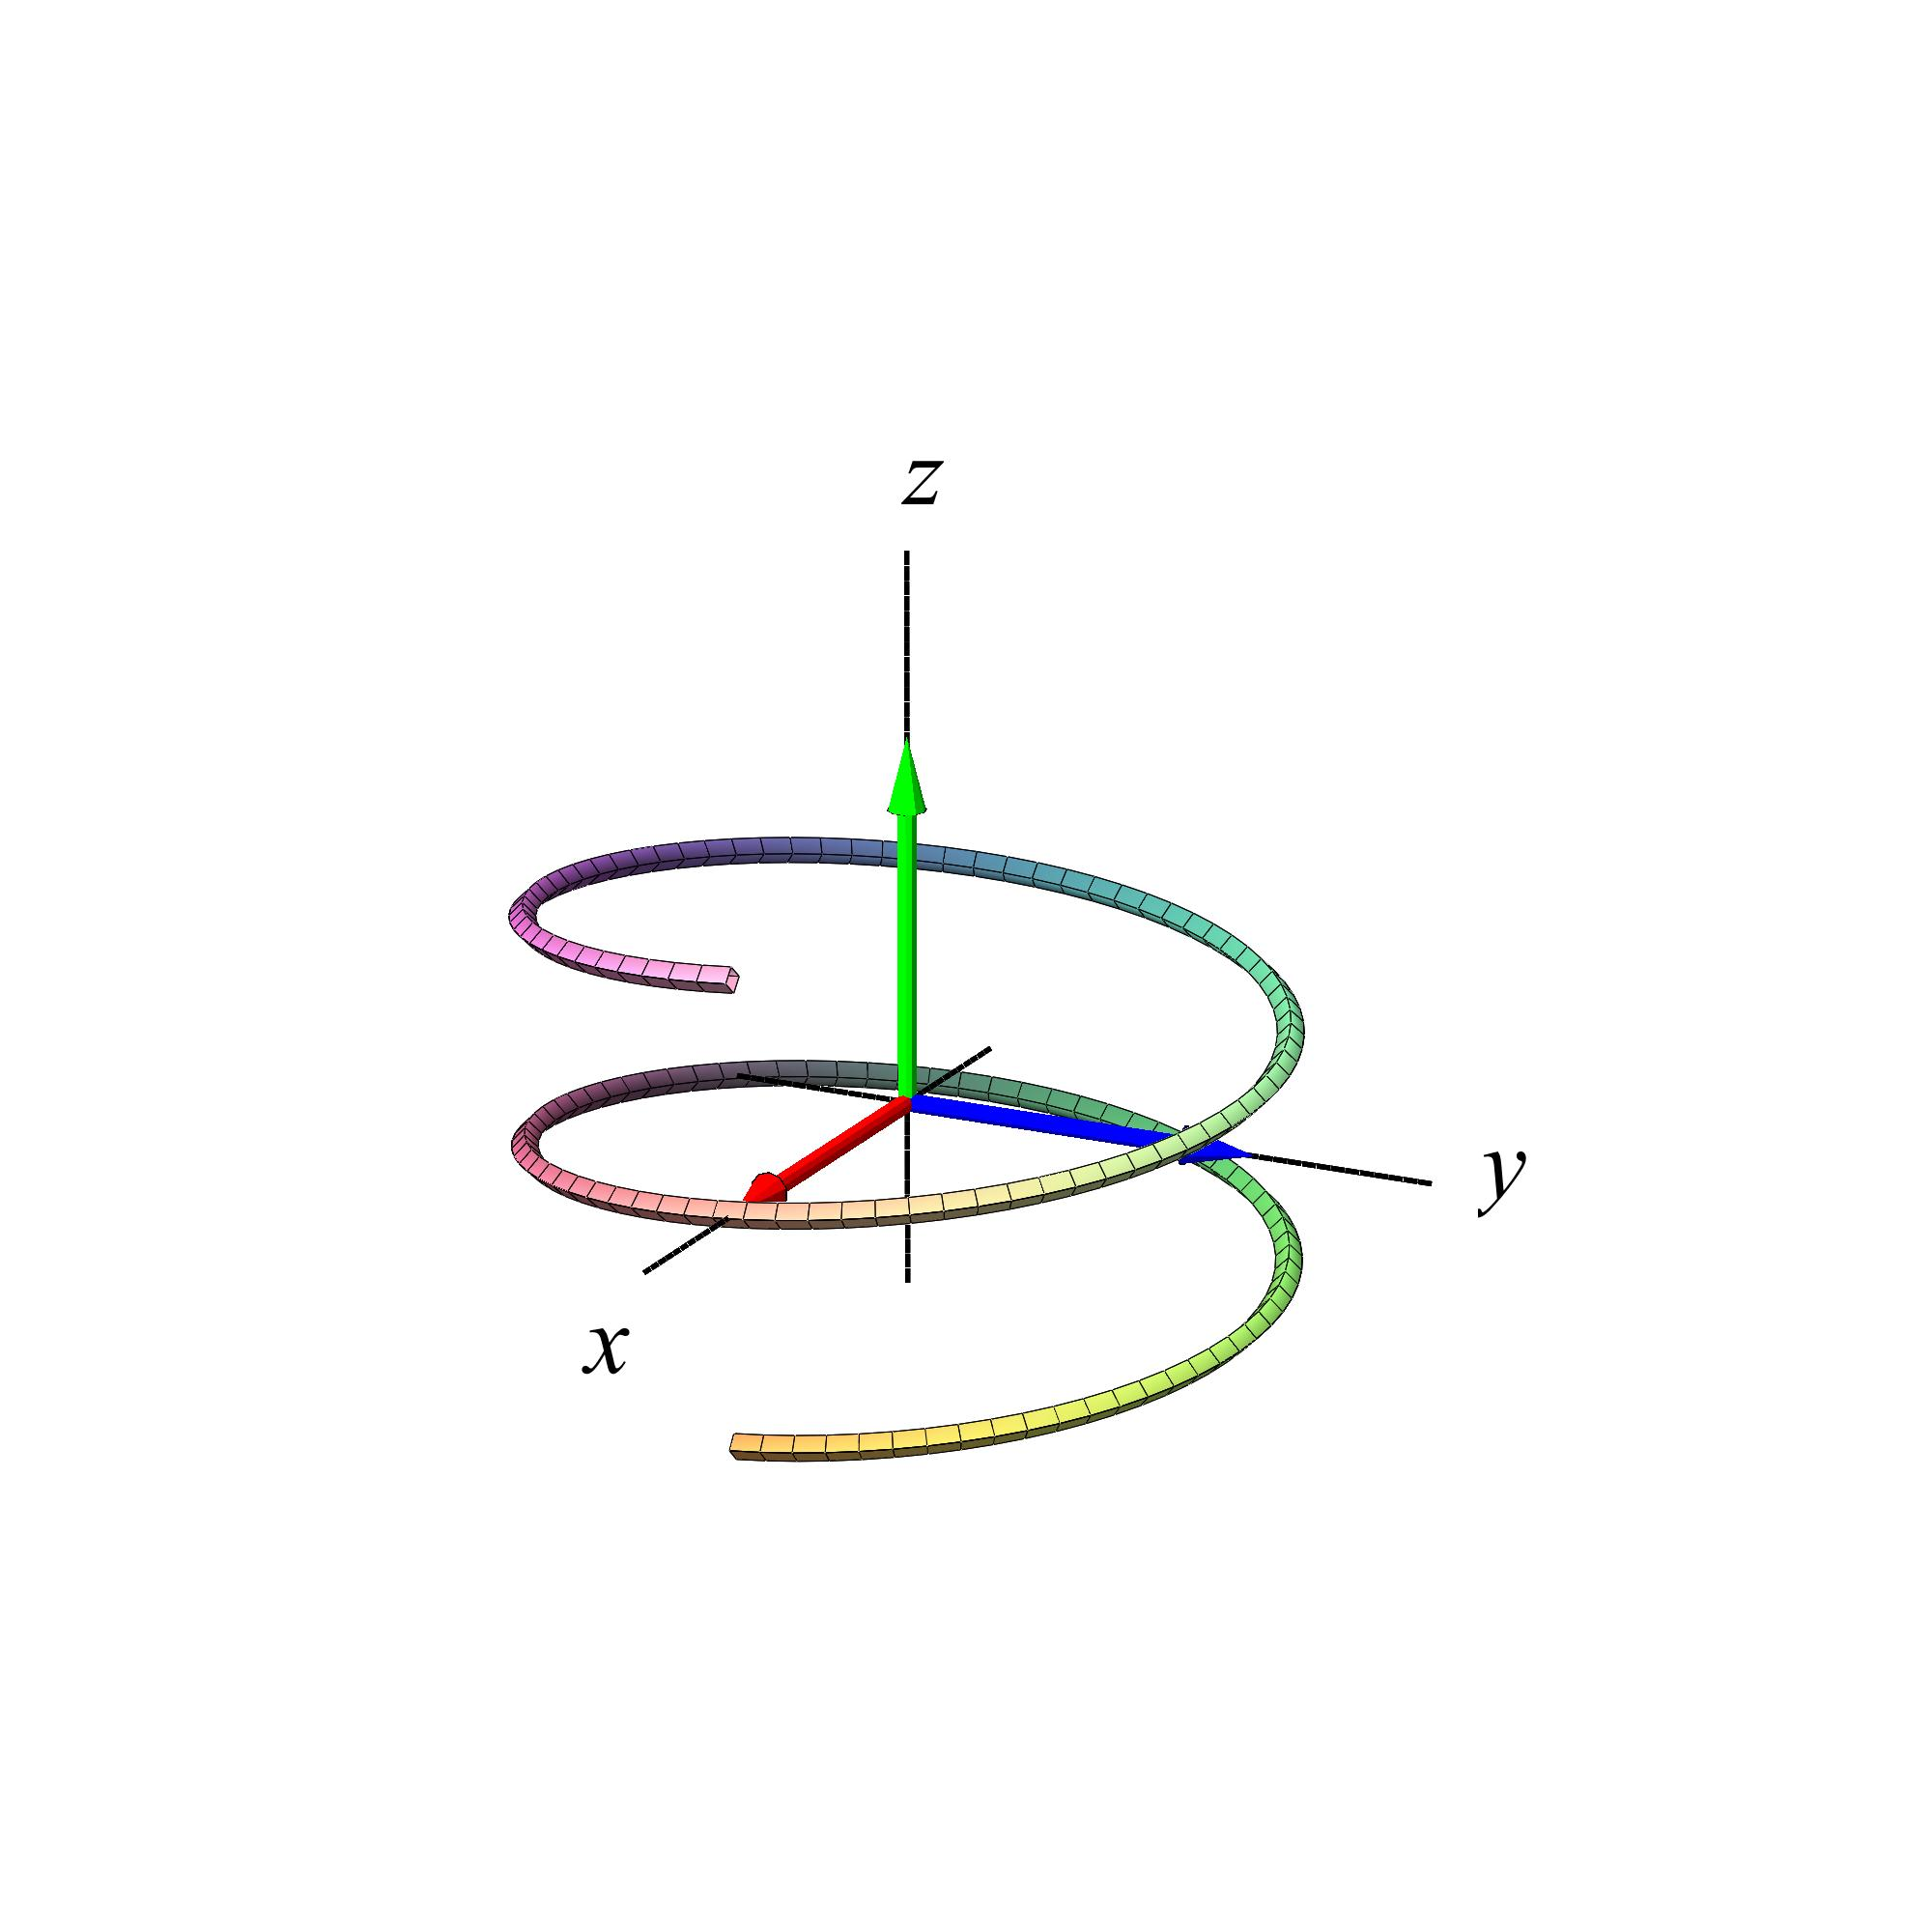
\includegraphics[height=70mm]{FIGS/plotTangKurve3}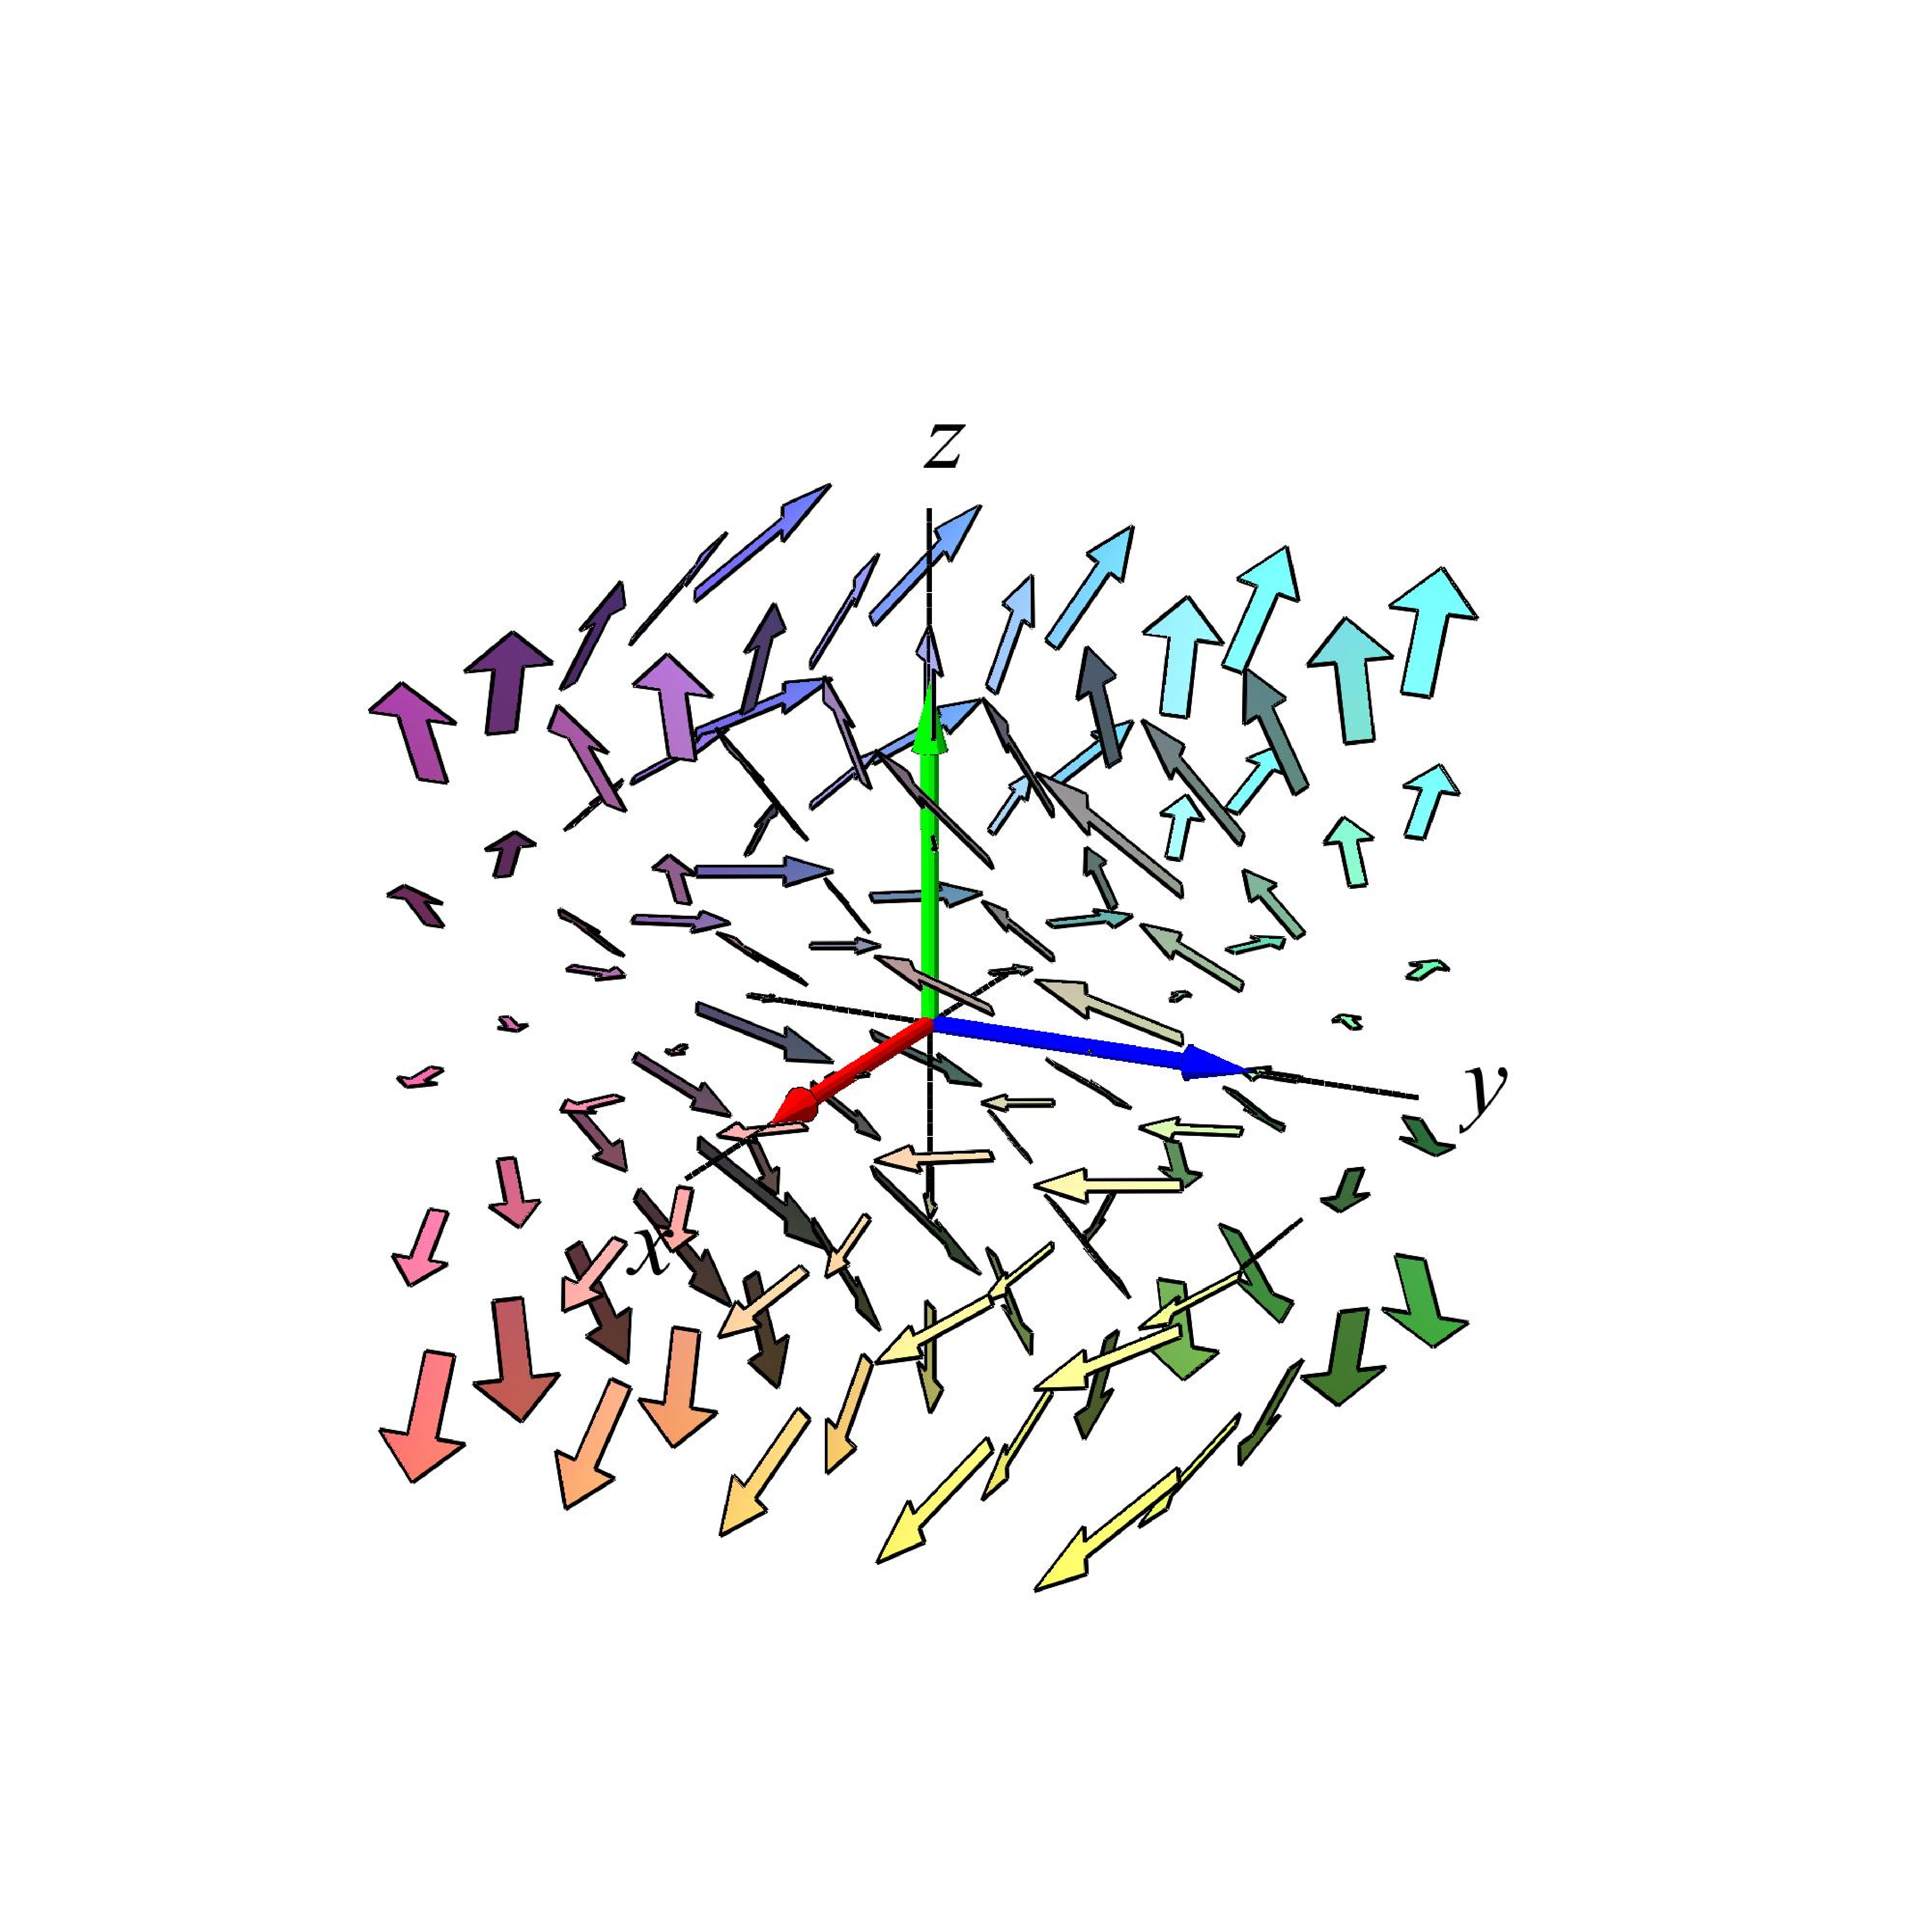
\includegraphics[height=70mm]{FIGS/plotTangKurve2}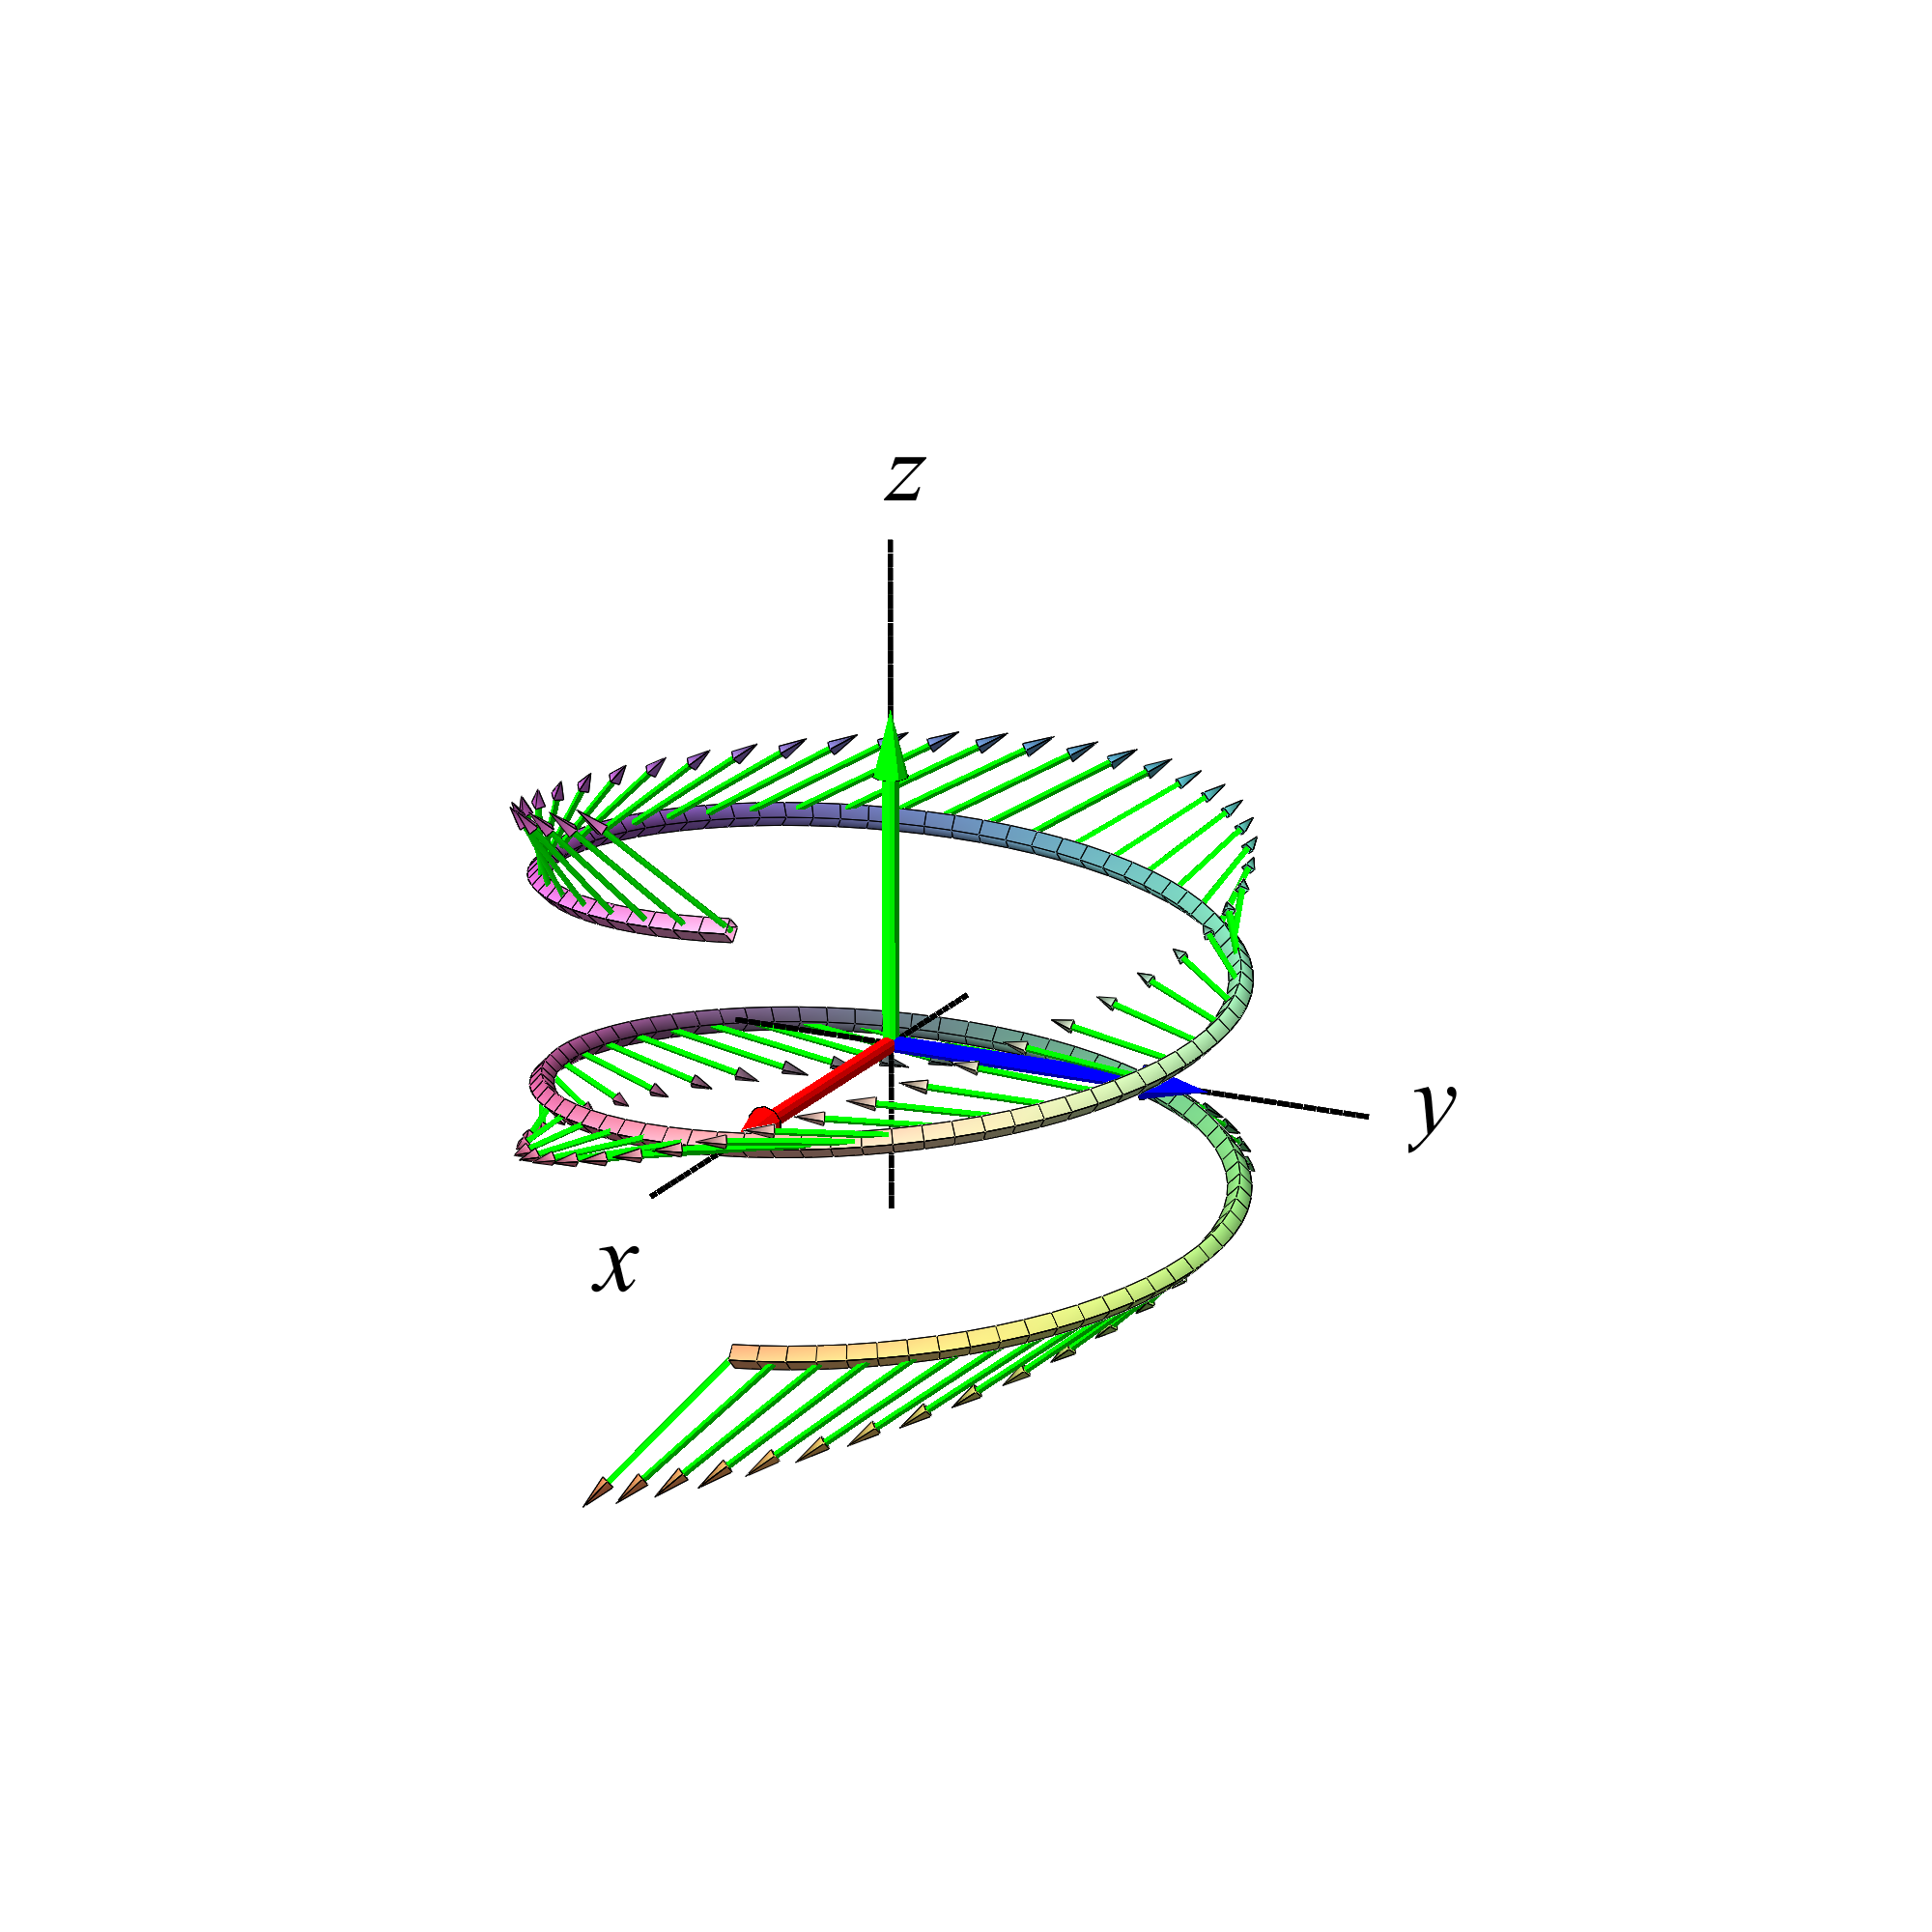
\includegraphics[height=70mm]{FIGS/plotTangKurve1}}
\begin{center}
\caption{\small{Skruelinjen ${\bf r}(u) \, = \,
\left(\cos(u), \,\sin(u),\, \frac{1}{10}u\right),
\, \, u \, \in [-2\pi, 2\pi]\,$, og vektorfeltet
$\, {\mathbf{V}}(x,y,z) \, = \, (x, -(x+y), 2z)\, $
er her antydet -- dels i rummet og dels langs skruelinjen.}} \label{figHelixVectors}
\end{center}
\end{figure}

\begin{method}[Tangentielle linjeintegraler til variabel punkt]\label{metodeTangKurveVar}
Lad $\mathbf{V}(x,y,z)$ være et givet vektorfelt i rummet. Vi vil nu konstruere en funktion $F^{*}(x,y,z)$ i rummet
som i punktet $(x_{0}, y_{0}, z_{0})$ er defineret til at være kurveintegralet af $\mathbf{V}(x,y,z)$ langs det rette linjestykke fra $(0,0,0)$ til punktet $(x_{0}, y_{0}, z_{0})$, dvs. $F^{*}$ defineres således:
\begin{equation}
F^{*}(x_{0}, y_{0}, z_{0}) = \Tan({\bf V}, K_{\bf r}) \quad ,
\end{equation}
hvor kurven er givet ved den simplest mulige kurve fra $(0,0,0)$ til $(x_{0}, y_{0}, z_{0})$:
\begin{equation}
K_{\bf r}: \,\, {\bf r}(u) \, = \,(u\cdot x_{0}, u\cdot y_{0},  u\cdot z_{0}) = u \cdot (x_{0}, y_{0}, z_{0}) \, , \, \, \, u \in
\left[ 0, 1\right]\quad .
\end{equation}
Så har vi dermed følgende funktionsværdier for (stjerne-)funktionen hørende til $\mathbf{V}(x,y,z)$:
\begin{equation} \label{eqIntFstar}
\begin{aligned}
F^{*}(x_{0}, y_{0}, z_{0}) &= \Tan({\bf V}, K_{\bf r}) \\
&=  \int_{0}^{1}{\bf V}({\bf r}(u))\bm{\cdot} {\bf r}'(u)\,\,du  \\
&=  (x_{0}, y_{0}, z_{0}) \bm{\cdot} \int_{0}^{1}{\bf V}(u\cdot x_{0}, u\cdot y_{0}, u\cdot z_{0}) \,\,du  \quad .
\end{aligned}
\end{equation}
Det sidste integral i (\ref{eqIntFstar}) skal forstås som et integral af hver af de tre koordinatfunktioner af ${\bf V}(u\cdot x_{0}, u\cdot y_{0}, u\cdot z_{0})$. Integralet giver dermed en vektor med tre komposanter sådan at skalarproduktet med stedvektoren $(x_{0}, y_{0}, z_{0})$ derefter giver en talværdi, som altså er værdien af $*$-funktionen $F^{*}(x,y,z)$ i $(x_{0}, y_{0}, z_{0})$.
\end{method}

\begin{example}[Konstruktion af tangentiel linjeintegral til variable punkt]\label{exampTangKurvVar}
Lad $\mathbf{V}(x,y,z)$ betegne følgende vektorfelt i rummet:
\begin{equation}
\mathbf{V}(x,y,z) = (x, 2y, 3z) \quad .
\end{equation}
Så er den tilhørende $*$-funktion:
\begin{equation}
\begin{aligned}
F^{*}(x_{0}, y_{0}, z_{0}) &= (x_{0}, y_{0}, z_{0}) \bm{\cdot} \int_{0}^{1}{\bf V}(u\cdot x_{0}, u\cdot y_{0}, u\cdot z_{0}) \,\,du  \\
&= (x_{0}, y_{0}, z_{0}) \bm{\cdot} \int_{0}^{1}(u\cdot x_{0}, 2u\cdot y_{0}, 3u\cdot z_{0})\,\,du  \\
&=  \frac{1}{2} \cdot (x_{0}, y_{0}, z_{0}) \bm{\cdot}(x_{0}, 2\cdot y_{0}, 3\cdot z_{0}) \\
&=   \frac{1}{2}\cdot\left(x_{0}^{2} + 2\cdot y_{0}^{2} +  3\cdot z_{0}^{2}\right) \\
&= \frac{1}{2}\cdot x_{0}^{2} +  y_{0}^{2} + \frac{3}{2}\cdot z_{0}^{2} \quad.
\end{aligned}
\end{equation}
\end{example}

\begin{aha}
Bemærk, at (stjerne-)funktionen $$F^{*}(x, y, z) = \frac{1}{2}\cdot x^{2} +  y^{2} + \frac{3}{2}\cdot x^{2}$$ som er konstrueret i
eksempel \ref{exampTangKurvVar} har følgende gradient, som netop er det vektorfelt vi begyndte med:
\begin{equation}
\bm{\nabla}F^{*}(x,y,z)  = (x, 2y, 3z)= \mathbf{V}(x,y,z) \quad.
\end{equation}
Det er ikke nogen tilfældighed! Vektorfeltet har rotationsvektorfelt $\operatorname{\bf{Rot}} = \mathbf{0}$,  og er derfor et gradientvektorfelt, som vi skal se i sætning \ref{thmStamfunk} nedenfor.
\end{aha}

\section{Stamfunktion til et gradientvektorfelt}

\begin{definition}[Stamfunktion for et gradientvektorfelt] \label{thmStamfunkGradFelt}
Lad $\mathbf{V}(x,y,z)$ være et glat vektorfelt i rummet. Hvis der findes en glat funktion $f(x,y,z)$ således at
\begin{equation}
\bm{\nabla}f(x,y,z) = \mathbf{V}(x,y,z) \quad ,
\end{equation}
så siges $f(x,y,z)$ at være en \emph{stamfunktion} til vektorfeltet $\mathbf{V}(x,y,z)$.
\end{definition}

\begin{think}
Hvis vi kender \'{e}n stamfunktion, så kender vi enhver af dem -- pånær en arbitrær konstant! Som vi skal se giver metode \ref{metodeTangKurveVar} en konstruktion af alle stamfunktioner til et givet vektorfelt. Hvis der \emph{ikke} findes nogen stamfunktion til vektorfeltet, så får vi ikke desto mindre alligevel med den metode konstrueret en $*$-funktion i rummet -- den funktion er imidlertid i så fald ikke nogen stamfunktion. Det kan og bør selvfølgelig afgøres ved at \emph{gøre prøve}, altså ved direkte at beregne gradienten af $*$-funktionen og sammenligne med det givne vektorfelt.
\end{think}


\begin{exercise}\label{exercStjerneOff}
Lad $\mathbf{V}(x,y,z)$ betegne vektorfeltet:
\begin{equation}
\mathbf{V}(x,y,z) = (x, 2y, 3z) \quad .
\end{equation}
bestem funktionsværdierne for (stjerne-)funktionen $F^{*}_{p}(x,y,z)$ ud fra det generelle punkt $p =(a,b,c)$ hørende til $\mathbf{V}(x,y,z)$.\\

Vink: Det rette linjestykke fra punktet $(a,b,c)$ til $(x_{0}, y_{0}, z_{0})$ kan parametriseres således:
\begin{equation}
K_{\bf r}: \,\, {\bf r}(u) \, = \,(a+ u\cdot (x_{0}-a), b+ u\cdot (y_{0}-b),  c+u\cdot ( z_{0}-c)) \, , \, \, \, u \in
\left[ 0, 1\right]\quad .
\end{equation}
således at
\begin{equation}
{\bf r}'(u) \, = \, (x_{0}-a), y_{0}-b,  z_{0}-c) \quad .
\end{equation}
Gælder det stadig, at
\begin{equation}
\bm{\nabla}F^{*}_{p}(x,y,z) = \mathbf{V}(x,y,z) \quad \textrm{?}
\end{equation}
\end{exercise}




\begin{theorem}[Tangentielt kurveintegral af et gradientvektorfelt] \label{thmGradTangInt}
Lad $f(x,y,z)$ betegne en glat funktion af de tre variable i rummet, og lad $\mathbf{V}(x,y,z) = \bm{\nabla}f(x,y,z)$ betegne gradientvektorfeltet for $f(x,y,z)$. Lad $K_{\mathbf{r}}$ være en glat parametriseret kurve fra et punkt $p$ til et punkt $q$ i rummet. Kurven behøver ikke nødvendigvis at være retlinjet. 

Så gælder følgende: Det tangentielle kurveintegral af  $\bm{\nabla}f(x,y,z)$ langs $K_{\mathbf{r}}$
afhænger kun af $p$ og $q$ og er uafhængig af kurven:
\begin{equation}
\Tan(\mathbf{V}, K_{\mathbf{r}}) = f(q) - f(p) \quad .
\end{equation}
\end{theorem}


\begin{bevis}
Vi bruger kædereglen fra \tref{NUID29-tn16}{eNote} på den sammensatte funktion $h(u) = f(\mathbf{r}(u))$ hvor $\mathbf{r}(u)$, $u \in \, ]u_{0}, u_{1}[$,  er en vilkårlig differentiabel kurve fra $p= (x_{0}, y_{0}, z_{0}) = \mathbf{r}(u_{0})$ til $q=(x_{1}, y_{1}, z_{1}) = \mathbf{r}(u_{1})$ og får derved:
\begin{equation}
h'(u) = \mathbf{r}'(u) \bm{\cdot} {\bm{\nabla}}f(\mathbf{r}(u)) \quad .
\end{equation}
Heraf følger, at $h(u)$  er en stamfunktion til funktionen på højresiden af ovenstående ligning:
\begin{equation} \label{eqIntegChainregelA}
h(u_{1}) - h(u_{0}) = \int_{u_{0}}^{u_{1}} \, \mathbf{r}'(u) \bm{\cdot} {\bm{\nabla}}f(\mathbf{r}(u))\, du  \quad .
\end{equation}
Men da
\begin{equation}
\begin{aligned}
h(u_{0}) &= f(\mathbf{r}(u_{0})) = f(p) \quad , \\
h(u_{1}) &= f(\mathbf{r}(u_{1})) = f(q) \quad ,
\end{aligned}
\end{equation}
får vi dermed
\begin{equation} \label{eqIntegChainregel}
\begin{aligned}
 f(q) &= f(p) + \int_{u_{0}}^{u_{1}} \,  \mathbf{r}'(u) \bm{\cdot} {\bm{\nabla}}f(\mathbf{r}(u)) \, du \\
 &= f(p) + \Tan(\mathbf{V}, K_{\mathbf{r}})  \quad ,
 \end{aligned}
\end{equation}
og det var det vi skulle vise.
\end{bevis}

\begin{aha}
Hvis kurven er lukket -- gerne sammensat af et endeligt antal glatte kurver som f.eks i en polygon med retlinede kanter --
får vi at det tangentielle kurveintegral af et gradientvektorfelt over den lukkede kurve er $0$.
\end{aha}

\begin{definition}[Cirkulationen af et vektorfelt langs en lukket kurve]\label{defCirkulation}
Lad $K_{\mathbf{r}}^{\circ}$ betegne en  \emph{lukket} kurve i rummet (som gerne kan være sammensat af et endeligt antal glatte kurver). Lad $\mathbf{V}(x,y,z)$ være et glat vektorfelt i rummet. Så kalder vi det tangentielle kurveintegral af $\mathbf{V}(x,y,z)$ over $K_{\mathbf{r}}^{\circ}$ \emph{cirkulationen} af $\mathbf{V}(x,y,z)$ over $K_{\mathbf{r}}^{\circ}$ og skriver:
\begin{equation}
\operatorname{Cirk}({\bf V}, K_{\bf r}^{\circ}) = \Tan({\bf V}, K_{\bf r}^{\circ}) \quad .
\end{equation}
\end{definition}

\begin{think}
Betegnelsen \emph{cirkulation} er helt rimelig. Hvis vektorfeltet er et gradientvektorfelt ved vi, at rotationen er $\mathbf{0}$ overalt, se \tref{NUID40-tn24}{eNote}, og det stemmer med, at cirkulationen i disse tilfælde også er $0$ for enhver lukket kurve.
\end{think}




\begin{figure}[t]
\centerline{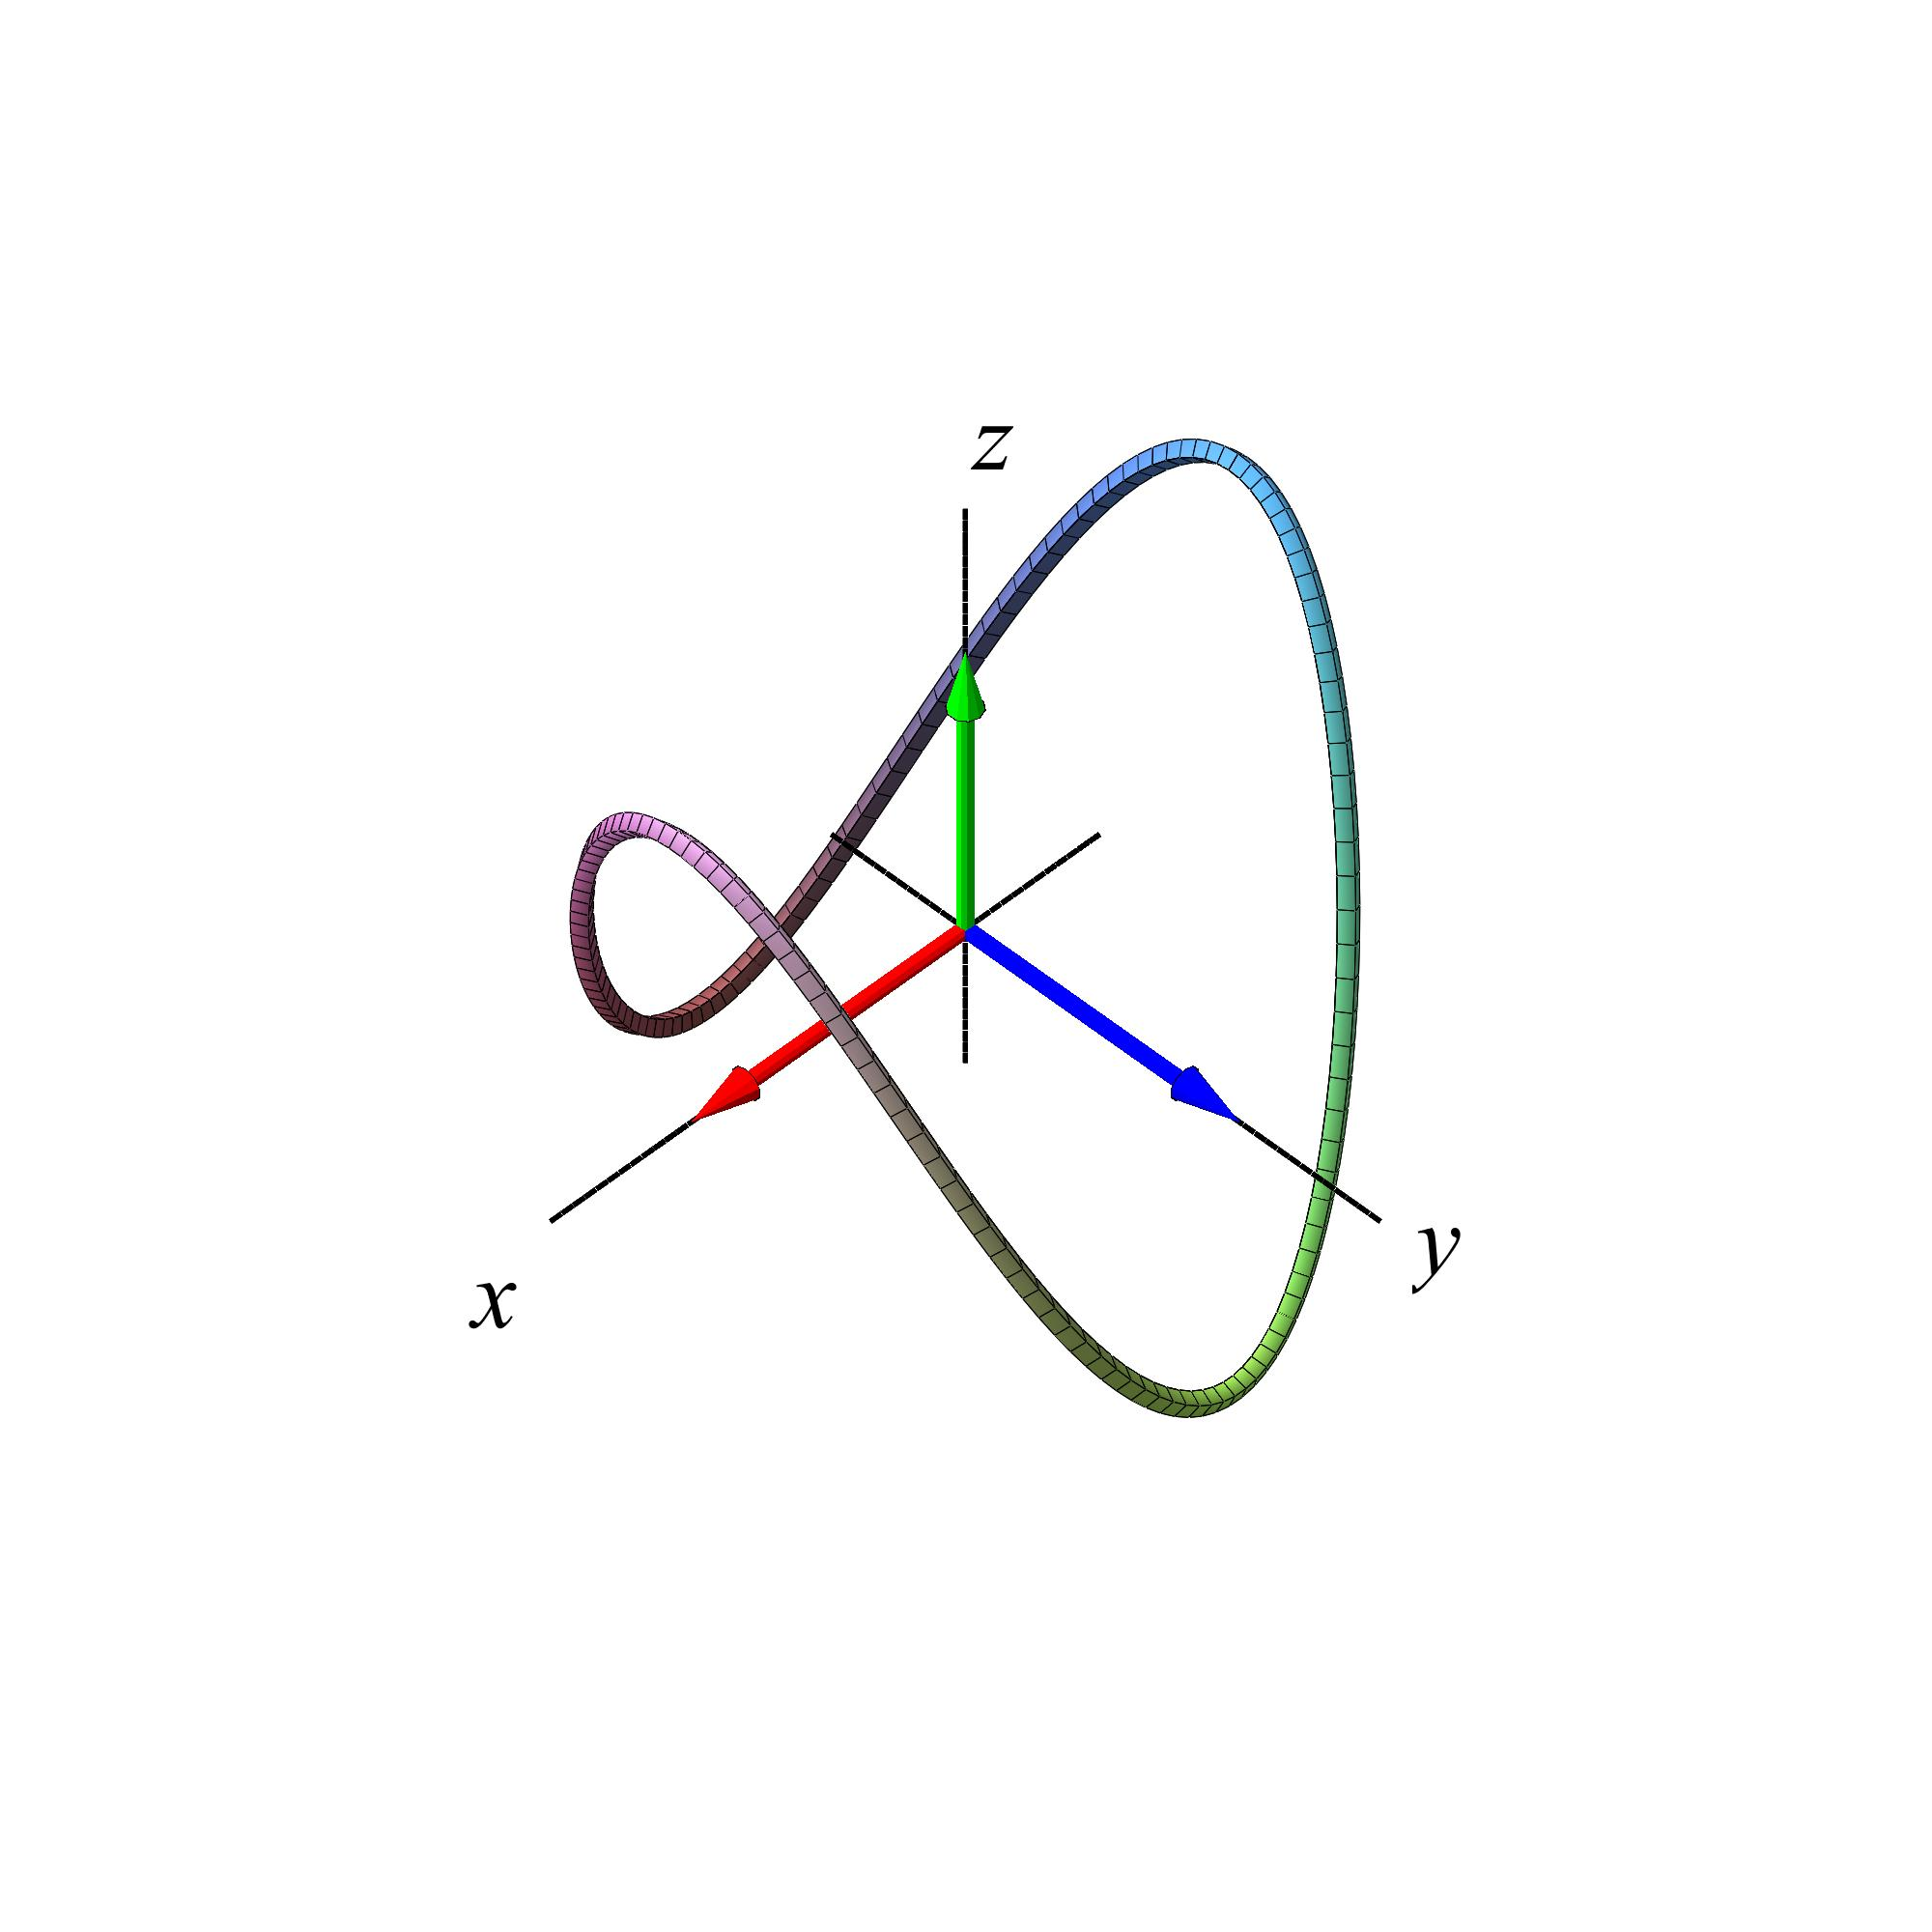
\includegraphics[height=70mm]{FIGS/plotTangKurveLuk1}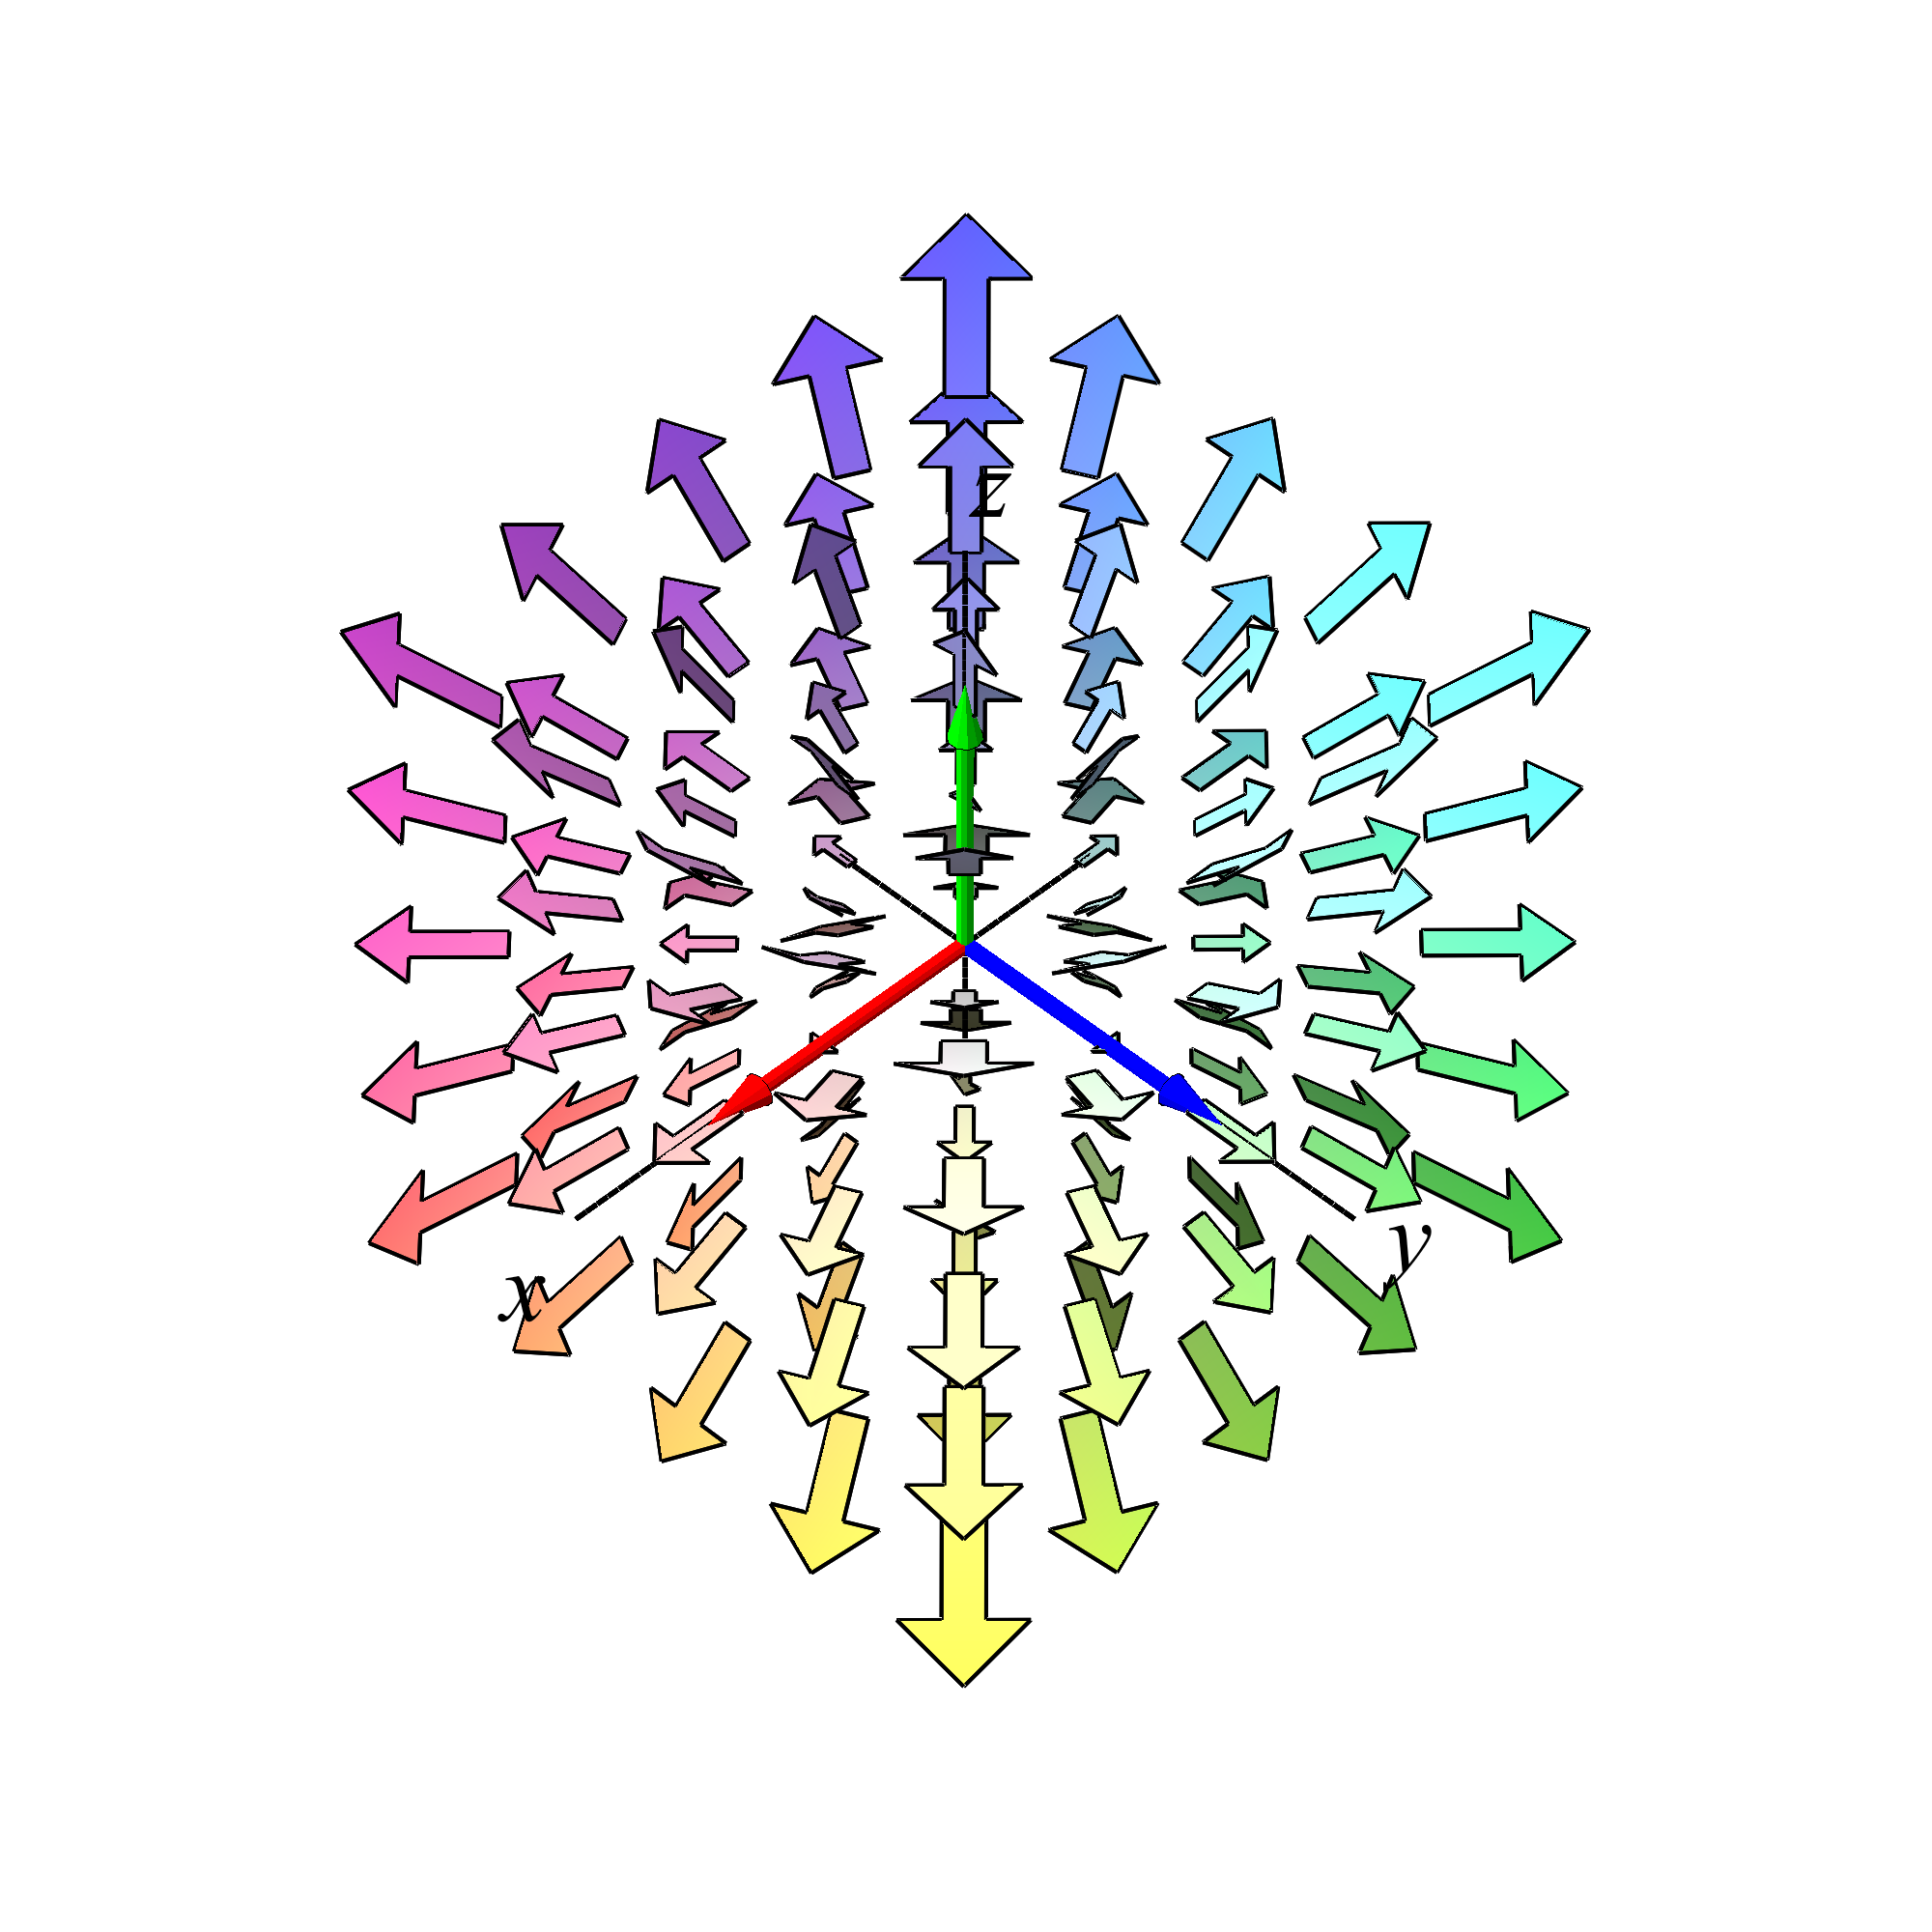
\includegraphics[height=70mm]{FIGS/plotTangKurveLuk2}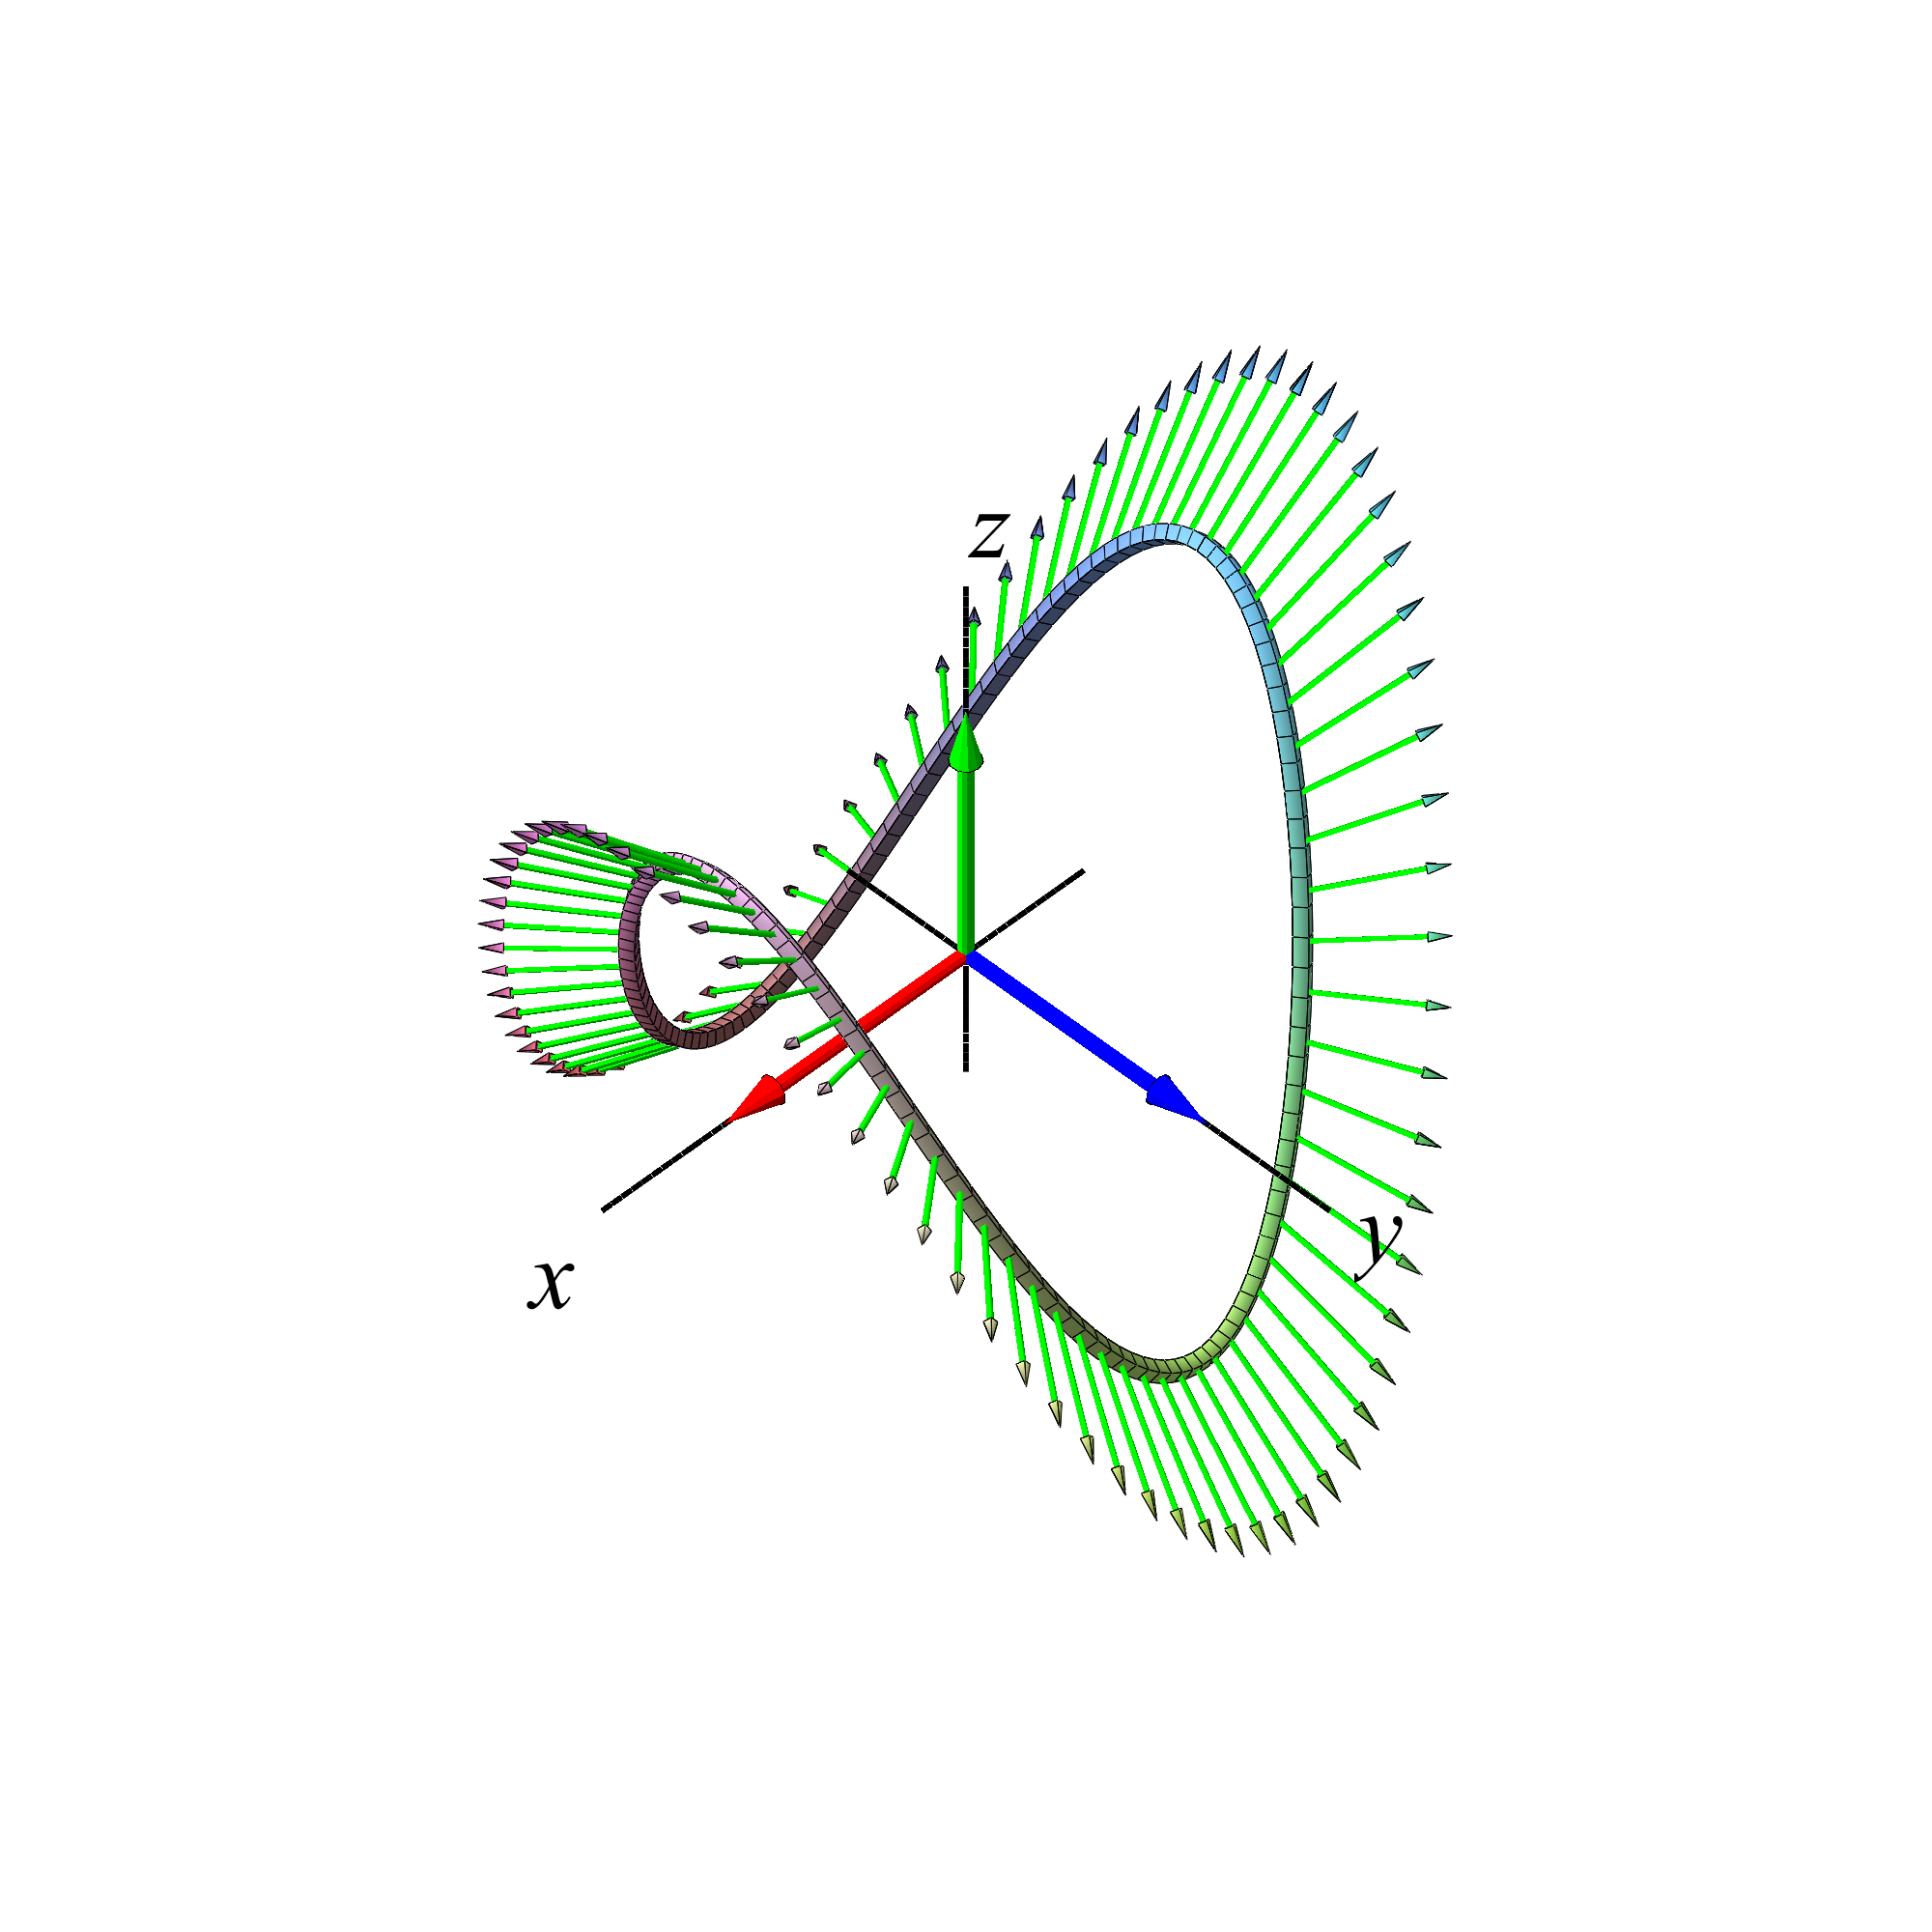
\includegraphics[height=70mm]{FIGS/plotTangKurveLuk3}}
\begin{center}
\caption{\small{Den lukkede kurve ${\bf r}(u) \, = \,
\left( \cos(t), \sin(t), \cos(2\cdot t) \right),
\, \, u \, \in [-\pi, \pi]\, $ og gradient-vektorfeltet
$\, {\mathbf{V}}(x,y,z) \, = \, (x, y,z)\,  = \, \bm{\nabla}f(x,y,z)$ for $f(x,y,z)= (x^{2} + y^{2} + z^{2})/2$
er her antydet -- dels i rummet og dels langs kurven. }} \label{figKurveLuk}
\end{center}
\end{figure}

Vi har allerede nu indset den ene halvdel af følgende sætning -- den anden (lidt vanskeligere) halvdel er bevist nedenfor:

\begin{theorem}[Cirkulationssætningen]\label{thmCirkulation}
Et glat vektorfelt $\mathbf{V}(x,y,z)$ i rummet er et gradientvektorfelt hvis og kun hvis der gælder:
\begin{equation}
\operatorname{Cirk}({\bf V}, K_{\bf r}^{\circ}) = 0
\end{equation}
for \emph{alle} lukkede kurver $K_{\mathbf{r}}^{\circ}$. \\

En stamfunktion kan konstrueres ved linjeintegralmetoden \ref{metodeTangKurveVar}.
\end{theorem}
\begin{bevis}
Som nævnt ved vi allerede, at hvis $\mathbf{V}(x,y,z)$ er et gradientvektorfelt, så er cirkulationen $0$ for enhver lukket kurve. Den anden vej handler altså om at antage, at alle lukkede kurver giver cirkulation $0$ og derudfra slutte, at så er det pågældende vektorfelt et gradientvektorfelt. Vi vil derfor konstruere en funktion $F(x,y,z)$ hvis gradientvektorfelt er det givne vektorfelt. Der er i ovenstående fremstilling stort set kun \'{e}n kandidat, der eventuelt ville kunne bruges som en sådan funktion, nemlig $*$-funktionen $F^{*}(x,y,z)$ hørende til $\mathbf{V}(x,y,z)$:
\begin{equation}
F^{*}(x,y,z) = (x,y,z)\bm{\cdot} \int_{0}^{1} \mathbf{V}(u\cdot x, u\cdot y, u\cdot z) \, du \quad.
\end{equation}
Da cirkulationen er $0$ langs enhver lukket kurve ved vi, at denne funktion ikke afhænger af integrationsvejen: Det tangentielle kurveintegral af $\mathbf{V}(x,y,z)$ langs enhver anden kurve fra $(0,0,0)$ til $(x,y,z)$ vil give samme værdi som $F^{*}(x,y,z)$. \\

Vi vil vise, at gradienten af $F^{*}(x,y,z)$ i punktet $(x_{0}, y_{0}, x_{0})$ er $\mathbf{V}(x_{0},y_{0},z_{0})$, så vi ser på
\begin{equation}\label{eqInt00}
F^{*}(x,y,z) = F^{*}(x_{0}, y_{0}, z_{0}) + \Tan(\mathbf{V}, K_{\mathbf{r}}) \quad,
\end{equation}
hvor $K_{\mathbf{r}}$ er en vilkårlig glat kurve fra (udviklings-)punktet $(x_{0}, y_{0}, z_{0})$ til et vilkårligt andet punkt $(x,y,z)$.
Vi vælger \emph{igen} det rette linjestykke mellem de to punkter:
\begin{equation}
K_{\mathbf{r}} \quad : \quad \mathbf{r}(u) = (x_{0}, y_{0}, z_{0}) + u\cdot ((x,y,z) - (x_{0}, y_{0}, z_{0})) \quad , \quad u \in [0,  1] \quad ,
\end{equation}
 og får så:
\begin{equation}\label{eqInt01}
\Tan(\mathbf{V}, K_{\mathbf{r}}) = (x-x_{0}, y-y_{0}, z-z_{0}) \bm{\cdot} \int_{0}^{1} \mathbf{V}(\mathbf{r}(u)) \, du
\end{equation}
Det første bidrag til dette skalarprodukt er
\begin{equation} \label{eqInt02}
(x-x_{0}) \cdot \int_{0}^{1} V_{1}(\mathbf{r}(u)) \, du \quad .
\end{equation}
Vi vil nu benytte den observation (se opgave \ref{exercIntMean}), at der for enhver glat funktion $g(u)$ på $[0, 1]$ gælder, at
der findes en værdi $\xi$ imellem $0$ og $1$ således at
\begin{equation}
\int_{0}^{1} g(u) \, du = g(\xi) \quad .
\end{equation}
Ved at bruge den integral-middelværdisætning får vi til indsættelse i (\ref{eqInt02}):
\begin{equation}
\begin{aligned}
&(x-x_{0}) \cdot \int_{0}^{1} V_{1}(\mathbf{r}(u)) \, du = (x-x_{0}) V_{1}(\mathbf{r}(\xi_{1})) \\
&= (x-x_{0}) \cdot \left(V_{1}(x_{0}, y_{0}, z_{0}) + \varepsilon_{1}(x-x_{0}, y-y_{0}, z-z_{0})\right) \quad ,
\end{aligned}
\end{equation}
idet $V_{1}(x, y, z) \to V_{1}(x_{0}, y_{0}, z_{0})$ for $(x,y,z) \to (x_{0}, y_{0}, z_{0})$. \\

Tilsvarende fås for de to andre bidrag til skalarproduktet i (\ref{eqInt01}), således at vi samlet har:
\begin{equation}
\begin{aligned}
\Tan(\mathbf{V}, K_{\mathbf{r}}) &= (x-x_{0}, y-y_{0}, z-z_{0}) \bm{\cdot} \left(\mathbf{V}(x_{0}, y_{0}, z_{0}) + \bm{\varepsilon}(x-x_{0}, y-y_{0}, z-z_{0})\right) \\
&= (x-x_{0}, y-y_{0}, z-z_{0})\bm{\cdot} \mathbf{V}(x_{0}, y_{0}, z_{0}) \\
&\phantom{(x-x_{0}, y-y_{0}, z-z_{0})}+ \rho_{(x_{0}, y_{0}, z_{0})}(x,y,z)\cdot {\varepsilon}(x-x_{0}, y-y_{0}, z-z_{0})
\end{aligned}
\end{equation}
Vi indsætter til sidst i (\ref{eqInt00}) og får følgende ligning
\begin{equation}
\begin{aligned}
F^{*}(x,y,z) &= F^{*}(x_{0}, y_{0}, z_{0}) + \Tan(\mathbf{V}, K_{\mathbf{r}}) \\
&= F^{*}(x_{0}, y_{0}, z_{0}) + (x-x_{0}, y-y_{0}, z-z_{0})\bm{\cdot} \mathbf{V}(x_{0}, y_{0}, z_{0}) \\
&\phantom{(x-x_{0}, y-y_{0}, z-z_{0})}+ \rho_{(x_{0}, y_{0}, z_{0})}(x,y,z)\cdot {\varepsilon}(x-x_{0}, y-y_{0}, z-z_{0})\quad.
\end{aligned}
\end{equation}
Gradienten af (stjerne-)funktionen $F^{*}(x,y,z)$ i $(x_{0}, y_{0}, z_{0})$  kan derefter aflæses ved direkte inspektion -- det er jo ''faktoren'' på
$(x-x_{0}, y-y_{0}, z-z_{0})$ før epsilon-leddet:
\begin{equation}
\bm{\nabla}F^{*}(x_{0},y_{0},z_{0}) = \mathbf{V}(x_{0}, y_{0}, z_{0}) \quad,
\end{equation}
hvilket netop betyder, at $\mathbf{V}(x, y, z)$ er et gradientvektorfelt (med $F^{*}(x,y,z)$ som stamfunktion), og det var det vi skulle vise.
\end{bevis}

\begin{exercise}\label{exercIntMean}
Overvej -- og indse -- den påstand vi har brugt i beviset for sætning \ref{thmCirkulation}:\\
For enhver glat funktion $g(u)$ på $[0, 1]$ gælder, at
der findes en værdi $\xi$ imellem $0$ og $1$ således at
\begin{equation}
\int_{0}^{1} g(u) \, du = g(\xi) \quad .
\end{equation}
\end{exercise}



 I analogi med cirkulationssætningen \ref{thmCirkulation} har vi ligeledes en to-vejs kobling mellem gradientvektorfelt-egenskaben  og \emph{rotation} $\mathbf{0}$:

\begin{theorem}[Stamfunktions-sætningen]\label{thmStamfunk}
Et glat vektorfelt $\mathbf{V}(x,y,z)$ i rummet er et gradientvektorfelt hvis og kun hvis der gælder:
\begin{equation}
\operatorname{\bf{Rot}}(\mathbf{V})(x,y,z) = (0,0,0) \quad . \quad
\end{equation}
En stamfunktion til vektorfeltet $\mathbf{V}(x,y,z)$  kan konstrueres ved linjeintegralmetoden \ref{metodeTangKurveVar}.
\end{theorem}
\begin{bevis}
Vi nøjes med at se på den ene (lette) vej -- rotationen af et gradientvektorfelt er $\mathbf{0}$.  Se også den påstand i
 \tref{NUID40-thmDivversRot}{sætning} i \tref{NUID40-tn24}{eNote}.
Lad altså $f(x,y,z)$ være en glat funktion i rummet. Så er
\begin{equation}
\bm{\nabla}f(x,y,z) = \left(f'_{x}(x,y,z), f'_{y}(x,y,z), f'_{z}(x,y,z) \right) \quad .
\end{equation}
Idet vi nøjes med at fokusere på første koordinat i  rotationsvektoren får vi heraf:
\begin{equation}
\begin{aligned}
\operatorname{\bf{Rot}}(\bm{\nabla}f)(x,y,z) &=
\left(\frac{\partial}{\partial y}f'_{z}(x,y,z) - \frac{\partial}{\partial z}f'_{y}(x,y,z), * , * \right) \\
&= \left(f''_{zy}(x,y,z) - f''_{yz}(x,y,z), * , *\right) \\
&= \left(0, *, * \right) \quad ,
\end{aligned}
\end{equation}
og tilsvarende $0$ for de to andre koordinater.
\end{bevis}


\begin{example}[Tangentielt kurveintegral af et ikke-gradientvektorfelt]\label{exampTangKurvRot}
Lad $\mathbf{V}(x,y,z) = (-y, x, 0)$. Så er  $\mathbf{V}(x,y,z)$ {\emph{ikke et gradientvektorfelt}} idet $\operatorname{\mathbf{Rot}}(\mathbf{V})(x,y,z) = (0,0,2) \neq (0,0,0)$, se også
\tref{NUID40-exampNonGradFelt}{eksempel} i  \tref{NUID40-tn24}{eNote}.\\

 Hvis vi vælger den lukkede kurve:
\begin{equation}
K_{\mathbf{r}} \quad : \quad \mathbf{r}(u) = (\cos(u), \sin(u), 0)  \quad , \quad u\in [-\pi, \pi] \quad ,
\end{equation}
får vi i overensstemmelse med cirkulationssætningen en cirkulation, der ikke er $0$:
\begin{equation}
\begin{aligned}
\Tan(\mathbf{V}, K_{\mathbf{r}}) &= \int_{-\pi}^{\pi} (- \sin(u), \cos(u), 0 )\bm{\cdot}(-\sin(u), \cos(u), 0)\, du \\
&= \int_{-\pi}^{\pi} \left( \sin^{2}(u) + \cos^{2}(u) \right)\, du \\
&= \int_{-\pi}^{\pi} \, 1 \, \, du \\
&= 2\cdot \pi \quad. \\
\end{aligned}
\end{equation}

Hvis vi konstruerer $*$-funktionen hørende til $\mathbf{V}(x,y,z) = (-y, x, 0)$ får vi en veldefineret funktion i rummet:
\begin{equation}
\begin{aligned}
F^{*}(x,y,z) &= (x,y,z)\bm{\cdot} \int_{0}^{1} \mathbf{V}(u\cdot x, u\cdot y,u\cdot z) \, du \\
&= (x,y,z)\bm{\cdot} \int_{0}^{1}( -u\cdot y, u\cdot x, 0) \, du \\
&= \frac{1}{2}\cdot \left( (x,y,z)\bm{\cdot} (-y, x, 0) \right) \\
&= 0 \quad ,
\end{aligned}
\end{equation}
og det er klart \emph{ikke}
en stamfunktion til $\mathbf{V}(x,y,z)$, hvilket er i fuld overensstemmelse med stamfunktionssætningen.
\end{example}





%%%%%%%%%%%%%%%%%%%%%%%%%%%%%%%%%%%%%%%%%%%%%%%%%%%
%%%%%%%%%%%%%%%%%%%%%%%%%%%%%%%%%%%%%%%%%%%%%%%%%%%
%%%%%%%%%%%%%%%%%%%%%%%%%%%%%%%%%%%%%%%%%%%%%%%%%%%
%%%%%%%%%%%%%%%%%%%%%%%%%%%%%%%%%%%%%%%%%%%%%%%%%%%






%%%%%%%%%%%%%%%%%%%%%%%%%%%%%%%%%%%%%%%%%%%%%%%%%%%%%%%%%%%%%
%%%%%%%%%%%%%%%%%%%%%%%%%%%%%%%%%%%%%%%%%%%%%%%%%%%%%%%%%%%%%
%%%%%%%%%%%%%%%%%%%%%%%%%%%%%%%%%%%%%%%%%%%%%%%%%%%%%%%%%%%%%

\begin{summary}
Vi har defineret det tangentielle kurveintegral for glatte vektorfelter langs glatte pa\-ra\-me\-tri\-se\-re\-de kurver
og vist, hvordan de tangentielle kurveintegraler kan benyttes til at konstruere stamfunktioner til et vektorfelt $\mathbf{V}(x,y,z)$ -- hvis ellers vektorfeltet er et gradientvektorfelt.
\begin{itemize}
\item Det tangentielle kurveintegral af ${\bf V}(x,y,z)$ langs den parametriserede kurve $K_{\bf r}$ kan beregnes således:
\begin{equation}
\Tan({\bf V}, K_{\bf r})\, = \, \int_{a}^{b}{\bf V}({\bf r}(u))\bm{\cdot} {\bf r}'(u)\,\,du \quad .
\end{equation}
Hvis kurven $K_{\bf r}$ er lukket, så betegnes kurven med $K_{\bf r}^{\circ}$, det tangentielle kurveintegral kaldes i så fald cirkulationen af vektorfeltet langs den lukkede kurve, og vi skriver
\begin{equation}
\operatorname{Cirk}(\mathbf{V}, K_{\bf r}^{\circ}) = \Tan(\mathbf{V}, K_{\bf r}^{\circ}) \quad .
\end{equation}
\item Stamfunktionssætningen giver en nødvendig og tilstrækkelig betingelse for at et givet vektorfelt er et gradientvektorfelt: \\

$\mathbf{V}(x,y,z)$ er et gradientvektorfelt hvis og kun hvis $\operatorname{\bf{Rot}}(\mathbf{V})(x,y,z)=(0,0,0)$. \\

\item Cirkulationssætningen udtrykker en tilsvarende nødvendig og tilstrækkelig betingelse for gradientfelt-egenskaben udtrykt ved cirkluationen af vektorfeltet langs lukkede kurver:\\

    $\mathbf{V}(x,y,z)$ er et gradientvektorfelt hvis og kun hvis $\operatorname{Cirk}(\mathbf{V}, K_{\bf r}^{\circ}) =0$ for alle lukkede kurver $K_{\bf r}^{\circ}$.\\

\item Stjerne-funktionen $F^{*}(x,y,z)$ hørende til et gradientvektorfelt $\mathbf{V}(x,y,z)$ er en stamfunktion til $\mathbf{V}(x,y,z)$. Funktionen beregnes som det tangentielle linjeintegral fra $(0,0,0)$ til punktet $(x,y,z)$ således:
    \begin{equation}
\begin{aligned}
F^{*}(x, y, z) &= \Tan({\bf V}, K_{\bf r}) \\
&=  \int_{0}^{1}{\bf V}({\bf r}(u))\bm{\cdot} {\bf r}'(u)\,\,du  \\
&=  (x, y, z) \bm{\cdot} \int_{0}^{1}{\bf V}(u\cdot x, u\cdot y, u\cdot z) \,\,du  \quad .
\end{aligned}
\end{equation}
\end{itemize}
\end{summary}


%%%%%%%%%%%%%%%%%%%%%%%%%%%%%%%%%%%%%%%%%%%%%
%%%%%%%%%%%%%%%%%%%%%%%%%%%%%%%%%%%%%%%%%%%%%
%%% HER SKAL DU STOPPE MED AT SKRIVE %%%%%%%%
%%%%%%%%%%%%%%%%%%%%%%%%%%%%%%%%%%%%%%%%%%%%%
%%%%%%%%%%%%%%%%%%%%%%%%%%%%%%%%%%%%%%%%%%%%%


\end{document} 

%%%%%%%%%%%%%%%%%%%%%%%%%%%%%%%%%%%%%%%%%%%%%%%%%%%
%%%%%%%%%%%%%%%%%%%%%%%%%%%%%%%%%%%%%%%%%%%%%%%%%%%

